\documentclass[a4paper,12pt,onecolumn]{article}

\usepackage[utf8]{inputenc}
\usepackage[english]{babel}
\usepackage{amssymb,amsmath,amsthm,array,epsfig,a4,verbatim,pstricks,url,subfig,hyperref}

\newtheorem{thm}{Theorem}
\newtheorem{lem}{Lemma}

\newcommand{\R}{{\mathbb R}}
\newcommand{\spa}{\operatorname{span}}
\newcommand{\vol}{\mathcal{L}^d}
\newcommand{\dH}[1]{\;{\rm d}{\cal H}^{#1}} % Hausdorff measure
\newcommand{\dL}[1]{\;{\rm d}{\cal L}^{#1}} % Lebesgue measure
\newcommand{\bigchi}{\ensuremath{\mathrm{\mathcal{X}}}}
\newcommand{\charfcn}[1]{\bigchi_{#1}} % characteristic function
\newcommand{\Vh}{\underline{V}(\Gamma^m)}
\newcommand{\Wh}{W(\Gamma^m)}
\newcommand{\Vht}{\underline{V}(\Gamma^h(t))}
\newcommand{\Wht}{W(\Gamma^h(t))}
\newcommand{\uspace}{\mathbb{U}}
\newcommand{\pspace}{\mathbb{P}}
\newcommand{\kspace}{\mathbb{K}}
\newcommand{\xspace}{\mathbb{X}}
\newcommand{\sigmaO}{o}
\newcommand{\nabs}{\nabla_{\!s}}
\newcommand{\Id}{I\!d}
\newcommand{\id}{\rm id}
\newcommand{\ddt}{\frac{\rm d}{{\rm d}t}}
\newcommand{\NbulkT}{\vec{N}_{\Gamma,\Omega}^T}
\newcommand{\Nbulk}{\vec{N}_{\Gamma,\Omega}} 
\newcommand{\errorXx}{\|\vec{X} - \vec{x}\|_{L^\infty}}
\newcommand{\LerrorUu}[1]{\|\vec U - I^h_{#1}\,\vec u\|_{L^2(\Omega_T)}}
\newcommand{\errorUu}[1]{\|\vec U - I^h_{#1}\,\vec u\|_{L^\infty}}
\newcommand{\errorPp}[1]{\|P - I^h_{#1}\,p\|_{L^\infty}}
\newcommand{\LerrorPp}[1]{\|P - I^h_{#1}\,p\|_{L^2(\Omega_T)}}
\newcommand{\unitn}{\vec{\rm n}}
\newcommand{\mat}[1]{\underline{\underline{#1}}\rule{0pt}{0pt}}

\renewcommand{\theequation}{\arabic{section}.\arabic{equation}}

%\textwidth 455pt \oddsidemargin 0pt \evensidemargin 0pt \headsep 0pt
%\headheight 0pt \textheight 655pt

\newif\ifthesis
%\thesistrue % comment in to add thesis parts

\title{Fitted Finite Element Discretization of Two--Phase Stokes Flow}
\author{Marco Agnese \and Robert N\"urnberg}

\begin{document}

\captionsetup[subfigure]{labelformat=empty} % remove label subplot
\newcolumntype{H}{>{\setbox0=\hbox\bgroup}c<{\egroup}@{}} % hide table column

\maketitle

\begin{abstract}
We propose a novel fitted finite element method for two-phase Stokes flow problems that uses piecewise linear finite elements to approximate the moving interface. The method can be shown to be unconditionally stable. Moreover, spherical stationary solutions are captured exactly by the numerical approximation. In addition, the meshes describing the discrete interface in general do not deteriorate in time, which means that in numerical simulations a smoothing or a remeshing of the interface mesh is not necessary. We present several numerical experiments for our numerical method, which demonstrate the accuracy and robustness of the proposed algorithm. 
\end{abstract}

\section{Introduction}\label{sec:introduction}
\textcolor{magenta}{TODO : explanation fitted mesh, pros and cons}
In this paper we want to compare the unfitted scheme for two--phase Stokes flow described in \cite{spurious} with our fitted scheme. See Figure~\ref{fig:meshes_uniform} and Figure~\ref{fig:meshes_adaptive} for two examples of 2D fitted meshes using an uniform and an adaptive meshing, respectively.  

\begin{figure}[htbp]
  \centering
  \subfloat[Stationary bubble problem]{\includegraphics[width=.45\textwidth]{figures/mesh_uniform.ps}}\quad
  \subfloat[Expanding bubble problem]{\includegraphics[width=.45\textwidth]{figures/mesh_hole_uniform.ps}}\\
  \caption{Initial fitted uniform 2D meshes with 32 interface elements.}
  \label{fig:meshes_uniform}
\end{figure}

\begin{figure}[htbp]
  \centering
  \subfloat[Stationary bubble problem]{\includegraphics[width=.45\textwidth]{figures/mesh_adaptive.ps}}\quad
  \subfloat[Expanding bubble problem]{\includegraphics[width=.45\textwidth]{figures/mesh_hole_adaptive.ps}}\\
  \caption{Initial fitted adaptive 2D meshes with 64 interface elements.}
  \label{fig:meshes_adaptive}
\end{figure}

\section{The two--phase Stokes problem}\label{sec:problem}

\textcolor{magenta}{TODO : add brief description of the fluidodynamics model, the meaning of the stress tensor and the menaing of the conditions on the interface, put a reference to the model}

In this paper we consider two--phase Stokes flow in a given domain $\Omega\subset\mathbb{R}^d$, where $d=2$ or $d=3$. The domain $\Omega$ contains two different immiscible, incompressible, viscous fluids (liquid-liquid or liquid-gas) which for all $t\in[0,T]$ occupy time dependent regions $\Omega_+(t)$ and $\Omega_-(t):=\Omega\setminus\overline{\Omega}_+(t)$ and which are separated by an interface $(\Gamma(t))_{t\in[0,T]}$, $\Gamma(t)\subset\Omega$. See Figure~\ref{fig:sketch} for an illustration.
\begin{figure}
\begin{center}
\unitlength15mm
\psset{unit=\unitlength,linewidth=1pt}
\begin{picture}(4,3.5)(0,0)
\psline[linestyle=solid]{-}(0,0)(4,0)(4,3.5)(0,3.5)(0,0)
\psccurve[showpoints=false,linestyle=solid] 
 (1,1.3)(1.5,1.6)(2.7,1.0)(2.5,2.6)(1.6,2.5)(1.1,2.7)
\psline[linestyle=solid]{->}(2.92,1.6)(3.4,1.6)
\put(3.25,1.7){{\black $\vec\nu$}}
\put(2.9,1.0){{$\Gamma(t)$}}
\put(2,2.1){{$\Omega_-(t)$}}
\put(0.5,0.5){{$\Omega_+(t)$}}
\end{picture}
\end{center}
\caption{The domain $\Omega$ in the case $d=2$.}
\label{fig:sketch}
\end{figure}
For later use, we assume that $(\Gamma(t))_{t\in [0,T]}$ is a sufficiently smooth evolving hypersurface without boundary that is parameterized by $\vec x(\cdot,t):\Upsilon\to\R^d$, where $\Upsilon\subset \R^d$ is a given reference manifold, i.e.\ $\Gamma(t) = \vec x(\Upsilon,t)$. Then
\begin{equation} \label{eq:V}
\vec{\mathcal{V}}(\vec z, t) := \vec x_t(\vec q, t) \qquad \forall\ \vec z = \vec x(\vec q,t) \in \Gamma(t)
\end{equation}
defines the velocity of $\Gamma(t)$, and $\vec{\mathcal{V}} \,.\,\vec{\nu}$ is the normal velocity of the evolving hypersurface $\Gamma(t)$,
where $\vec\nu(t)$ is the unit normal on $\Gamma(t)$ pointing into $\Omega_+(t)$.

In order to define the model, we introduce the stress tensor $\mat\sigma : \Omega \times [0,T] \to \R^{d \times d}$
\begin{equation} \label{eq:stress_tensor}
\mat\sigma = \mu \,(\nabla\,\vec u + (\nabla\,\vec u)^T) - p\,\mat\id = 2\,\mu\, \mat D(\vec u)-p\,\mat\id\,,
\end{equation}
where $\vec u : \Omega \times [0, T] \to \R^d$ is the fluid velocity, $p : \Omega \times [0, T] \to \R$ is the pressure and $\mu(t) = \mu_+\,\charfcn{\Omega_+(t)} + \mu_-\,\charfcn{\Omega_-(t)}$, with $\mu_\pm \in \R_{>0}$, denotes the dynamic viscosities in the two phases.
 
We denote the identity matrix as $\mat\id \in \R^{d \times d}$, $\mat D(\vec u):=\frac12\, (\nabla\vec u+(\nabla\vec u)^T)$ is the rate-of-deformation tensor and $\charfcn{\mathcal{A}}$ defines the characteristic function for a set $\mathcal{A}$.

For low Reynolds numbers one can neglect the inertia terms, and so the equations governing the fluid are 
\begin{subequations}
\begin{alignat}{2}
- \nabla\,.\,\mat\sigma & = \vec f \qquad &&\mbox{in } \Omega_\pm(t)\,, \label{eq:stokes_momentum} \\
\nabla\,.\,\vec u & = 0 \qquad &&\mbox{in } \Omega_\pm(t)\,, \label{eq:stokes_mass}   
\end{alignat}
\end{subequations}
where $\vec f : \Omega \times [0, T] \to \R^d$ is the forcing term.

On the free surface $\Gamma(t)$, the following conditions need to hold:
\begin{subequations}
\begin{alignat}{2}
[\vec u]_-^+ & = \vec 0 \qquad &&\mbox{on } \Gamma(t)\,, \label{eq:interface_jump_velocity} \\ 
[\mat\sigma\,\vec \nu]_-^+ & = -\gamma\,\varkappa\,\vec\nu \qquad &&\mbox{on } \Gamma(t)\,, \label{eq:interface_jump_stress} \\ 
\mathcal{V} &= \vec u\,.\,\vec \nu \qquad &&\mbox{on } \Gamma(t)\,, \label{eq:interface_velocity} 
\end{alignat}
\end{subequations}
where $\gamma>0$ is the surface tension coefficient and $\varkappa$ denotes the mean curvature of $\Gamma(t)$, i.e.\ the sum of the principal curvatures of $\Gamma(t)$, where we have adopted the sign convention that $\varkappa$ is negative where $\Omega_-(t)$ is locally convex. To close the system we prescribe the initial data $\Gamma(0) = \Gamma_0$ and the boundary condition $\vec u = \vec 0$ on $\partial \Omega$. We note that (\ref{eq:interface_velocity}) can be rewritten as
\begin{equation} \label{eq:interface_velocity_bis} 
(\vec{\mathcal{V}}-\vec u)\,.\,\vec{\nu} = 0 \qquad \mbox{on } \Gamma(t)\, .
\end{equation}

Moreover, as usual, $[\vec u]_-^+ := \vec u_+ - \vec u_-$ and $[\mat\sigma\,\vec\nu]_-^+ := \mat\sigma_+\,\vec\nu - \mat\sigma_-\,\vec\nu$ denote the jumps in velocity and normal stress across the interface $\Gamma(t)$. Here and throughout, we employ the shorthand notation $\vec g_\pm := \vec g\!\mid_{\Omega_\pm(t)}$ for a function $\vec g : \Omega \times [0,T] \to \R^d$; and similarly for scalar and matrix-valued functions.

Therefore the total system can be rewritten as
\begin{subequations}
\begin{alignat}{2}
-2 \mu\,\nabla\,.\,\mat D(\vec u)+ \nabla\,p & = \vec f \quad &&\mbox{in } \Omega_\pm(t)\,, \label{eq:full_momentum} \\
\nabla\,.\,\vec u & = 0 \quad &&\mbox{in } \Omega_\pm(t)\,, \label{eq:full_mass} \\
\vec u & = \vec 0 \qquad &&\mbox{on } \partial\Omega\,, \label{eq:full_initial_velocity} \\
[\vec u]_-^+ & = \vec 0 \quad &&\mbox{on } \Gamma(t)\,, \label{eq:full_jump_velocity} \\ 
[2\mu \,\mat D(\vec u)\,.\,\vec\nu - p\,\vec \nu]_-^+ & = -\gamma\,\varkappa\,\vec\nu \quad &&\mbox{on } \Gamma(t)\,, \label{eq:full_jump_stress} \\ 
(\vec{\mathcal{V}}-\vec u)\,.\,\vec{\nu} & = 0 \quad &&\mbox{on } \Gamma(t)\,,\label{eq:full_velocity}  \\
\Gamma(0) & = \Gamma_0 \,,\label{eq:full_initial_interface} 
\end{alignat}
\end{subequations}
which is appropriate for the weak formulation considered in this paper. 

\ifthesis
We can notice that for the one--phase Stokes flow, $\mu_+=\mu_-=\mu$, using the incompressibility condition (\ref{eq:full_mass}) we have
\begin{equation}
\nabla\,.\,\mat D(\vec u) = \nabla\,.\big(\nabla\vec u+(\nabla\vec u)^T\big) = \Delta \vec u + \nabla(\nabla\,.\vec u) = \Delta u
\end{equation}
therefore the system (\ref{eq:full_momentum}-\ref{eq:full_mass}) can be rewritten as
\begin{equation}
- \mu\,\Delta\vec u+\nabla\,p  = \vec f, \qquad \nabla\,.\,\vec u = 0 \qquad \mbox{in } \Omega
\end{equation}
which is the canonical form of the one--phase Stokes problem.
\fi

\section{Energy bound and fluid volumes} \label{sec:volume_conservation}
\setcounter{equation} 0

\textcolor{magenta}{TODO : explain (\ref{eq:weak_stress_tensor})}

First of all an a priori energy bound holds and the numerical scheme should preserve it. We start noting that for the left hand side of (\ref{eq:stokes_momentum}) holds, $\forall \ \vec \xi \in H^1_0(\Omega, \R^d)$, the identity 
\begin{equation}\label{eq:weak_stress_tensor}
\int_{\Omega_+(t)\cup\Omega_-(t)} (\nabla\,.\,\mat\sigma)\,.\, \vec \xi \dL{d}  = - \int_{\Omega} \mat\sigma : \nabla\,\vec \xi \dL{d}
- \int_{\Gamma(t)} [\mat\sigma\,\vec\nu]_-^+\, . \,\vec \xi  \dH{d-1}.
\end{equation}
Here and throughout, $\mathcal{L}^d$ and $\mathcal{H}^{d-1}$ denote the Lebesgue measure in $\R^d$ and the $(d-1)$-dimensional Hausdorff measure, respectively. Using (\ref{eq:stress_tensor}) and (\ref{eq:interface_jump_stress}), we have that
\begin{align}
& - \int_{\Omega} \mat\sigma : \nabla\,\vec \xi \dL{d} - \int_{\Gamma(t)} [\mat\sigma\,\vec\nu]_-^+\, . \,\vec \xi  \dH{d-1} = \nonumber\\
&\int_{\Omega} \left( p\,\nabla\,.\,\vec \xi -2\,\mu\,\mat D(\vec u) : \mat D(2\vec \xi) \right) \dL{d} + \gamma \int_{\Gamma(t)} \varkappa\,\vec \nu \,.\, \vec \xi \dH{d-1}.
\end{align}
Choosing $\vec \xi=\vec u$ then gives, on recalling (\ref{eq:stokes_mass}),
\begin{equation}\label{eq:sigmaibp}
\int_{\Omega_+(t)\cup\Omega_-(t)} (\nabla\,.\,\mat\sigma)\,.\, \vec u \dL{d} = -\int_{\Omega} 2\,\mu\,\mat D(\vec u) : \mat D(\vec u) \dL{d} + \gamma \int_{\Gamma(t)} \varkappa\,\vec \nu \,.\, \vec u \dH{d-1}.
\end{equation}
 Then using the identity, see \cite[Lemma~2.1]{DeckelnickDE05}, 
\begin{equation}\label{eq:dtarea}
\ddt\,\mathcal{H}^{d-1}(\Gamma(t)) = -\int_{\Gamma(t)} \varkappa\,\mathcal{V} \dH{d-1} \,, 
\end{equation}
we obtain from (\ref{eq:sigmaibp}) that
\begin{align}
& \gamma\,\ddt\,\mathcal{H}^{d-1}(\Gamma(t)) = -\gamma \int_{\Gamma(t)} \varkappa\,\vec \nu \,.\,\vec u \dH{d-1} \nonumber\\
& \qquad =-2\int_\Omega\mu\, \mat D(\vec u):\mat D(\vec u) \dL{d} +\int_\Omega \vec f\,.\, \vec u \dL{d}\,.\label{eq:length}
\end{align}

Finally we show that during the evolution of the two--phase Stokes flow the fluid volumes are conserved. Indeed, due to the incompressibility condition, the volume of the two fluids is preserved since from (\ref{eq:full_mass},\ref{eq:full_velocity}) we have that
\begin{align}
\ddt \vol(\Omega_-(t)) & = \int_{\Gamma(t)} \mathcal{V}\dH{d-1}=\int_{\Gamma(t)}\vec u\,.\,\vec\nu \dH{d-1} \nonumber \\ 
& = \int_{\Omega_-(t)} \nabla\,.\,\vec u \dL{d} =0\,. \label{eq:conserved}
\end{align}
It will be our aim to introduce a fitted FEM for two--phase Stokes flow that satisfies discrete analogous of (\ref{eq:length}) and (\ref{eq:conserved}).

\section{Interface treatment}
\setcounter{equation} 0

As said in Section~\ref{sec:problem} we use an explicit method known as parametric approach to treat the interface. It involves seeking a parametrization over a base manifold. All the geometrical quantities of the hypersurface (e.g. curvature) can be expressed as derivatives of the parametrization.

In order to compute a discrete version of the mean curvature for polyhedral surfaces, we will use the identity
\begin{equation} \label{eq:LBop}
\Delta_s\, \vec \id = \varkappa\, \vec\nu \qquad \mbox{on $\Gamma(t)$}\,,
\end{equation}
where $\Delta_s = \nabs\,.\,\nabs$ is the Laplace--Beltrami operator on $\Gamma(t)$ with $\nabs\,.\,$ and $\nabs$ denoting surface divergence and surface gradient on $\Gamma(t)$, respectively. 

Precisely, $\nabla_s$ is the tangential gradient defined as
\begin{equation}\label{eq:tangent_gradient}
 \nabla_s f(\vec{p})=\nabla f(\vec{p})-\nabla f(p)\,.\,\vec{\nu}(\vec{p})\,\vec{\nu}(\vec{p}),\qquad \vec{p}\in\Gamma(t),
\end{equation}
for a smooth function $f$ defined in a neighbourhood of $\Gamma(t)$. 

It is possible to use a weak formulation of this identity discretizing directly the vector quantity $\vec\varkappa:=\varkappa\,\vec\nu$, see in \cite{Dziuk91,Bansch01,GanesanMT07}. Instead we follow the approach introduced in \cite{triplej} for $d=2$ and in \cite{gflows3d} for
$d=3$ which treats the mean curvature as a scalar and we discretize it separately from the normal $\vec\nu$. This approach leads to good mesh property and to a smaller algebraic system.

\section{Weak formulation}\label{sec:weak_formulation}
\setcounter{equation} 0

\textcolor{magenta}{TODO : explain that the surface gradient is the usual gradient}

In order to obtain a weak formulation, we define the function spaces
\begin{align*}
\uspace &:= H^1_0(\Omega, \R^d)\,,\qquad \pspace := L^2(\Omega)\,, \qquad \widehat\pspace := \{\eta\in\pspace : \int_\Omega\eta\dL{d}=0 \}\,,\\
\xspace &:= H^1(\Upsilon,\R^d) \qquad\mbox{and}\qquad \kspace := L^2(\Upsilon,\R)\,, 
\end{align*}  
and let $(\cdot,\cdot)$ and $\langle \cdot, \cdot \rangle_{\Gamma(t)}$ denote the $L^2$--inner products on $\Omega$ and $\Gamma(t)$, respectively. On recalling (\ref{eq:sigmaibp}) and using also (\ref{eq:LBop}), a possible weak formulation of (\ref{eq:full_momentum}--g) is then given as follows. Find the interface $\Gamma(t)$ and time dependent functions $\vec u$, $p$ and $\varkappa$ such that $\vec u(\cdot,t) \in \uspace$, $p(\cdot,t) \in \widehat\pspace$, $\varkappa(\cdot,t) \in \kspace$ and

\begin{subequations}
\begin{align}
& 2\left(\mu\,\mat D(\vec u), \mat D(\vec \xi)\right) - \left(p, \nabla\,.\,\vec \xi\right) - \gamma\,\left\langle \varkappa\,\vec\nu, \vec\xi\right\rangle_{\Gamma(t)} = \left(\vec f, \vec \xi\right)\quad \forall\ \vec\xi \in \uspace \,, \label{eq:weaka}\\
& \left(\nabla\,.\,\vec u, \varphi\right) = 0 \quad \forall\ \varphi \in \widehat\pspace\,, \label{eq:weakb} \\
&  \left\langle \vec{\mathcal{V}} - \vec u, \chi\,\vec\nu \right\rangle_{\Gamma(t)} = 0 \quad \forall\ \chi \in \kspace\,, \label{eq:weakc} \\
& \left\langle \varkappa\,\vec\nu, \vec\eta \right\rangle_{\Gamma(t)} + \left\langle \nabs\,\vec \id, \nabs\,\vec \eta \right\rangle_{\Gamma(t)}
= 0  \quad \forall\ \vec\eta \in \xspace\,\label{eq:weakd}
\end{align}
\end{subequations}
holds for almost all times $t \in (0,T]$, as well as the initial condition (\ref{eq:full_initial_interface}). Here we have observed that if $p \in \pspace$ is part of a solution to (\ref{eq:full_momentum}--g), then so is $p + c$ for an arbitrary $c\in \R$. Moreover, we note that for convenience we have adopted a slight abuse of notation in (\ref{eq:weaka}--d). In particular, in this paper we will identify functions defined on the reference manifold $\Upsilon$ with functions defined on $\Gamma(t)$. That is, we identify $v \in \kspace$ with $v \circ \vec{x}^{-1}$ on $\Gamma(t)$, where we recall that $\Gamma(t) = \vec{x}(\Upsilon,t)$, and we denote both functions simply as $v$. For example, $\vec{x} \equiv \vec \id$ is also the identity function on $\Gamma(t)$.

\section{Finite element approximation}\label{sec:fem}
\setcounter{equation} 0

We consider the partitioning  $0= t_0 < t_1 < \ldots < t_{M-1} < t_M = T$ of $[0,T]$ into possibly variable time steps $\tau_m := t_{m+1}-t_m$, $m=0 ,\ldots, M-1$ and the regular partitioning ${\cal T}^m$, $\forall m\ge 0$, of the domain $\Omega$ into disjoint open simplices $\sigmaO^m_j$, $j = 1 ,\ldots, J^m_\Omega$. 

On ${\cal T}^m$ we define the finite element spaces
\begin{equation*} 
 S^m_k := \{\chi \in C(\overline{\Omega}) : \chi\!\mid_{\sigmaO^m} \in \mathcal{P}_k(\sigmaO^m) \ \forall\ \sigmaO^m \in {\cal T}^m\} \subset H^1(\Omega),\quad k \in \mathbb{N}\,,
\end{equation*}
where $\mathcal{P}_k(\sigmaO^m)$ denotes the space of polynomials of degree $k$ on $\sigmaO^m$. Moreover, $S^m_0$ is the space of piecewise constant functions on ${\cal T}^m$.

Let $\uspace^m\subset\uspace$ and $\pspace^m\subset\pspace$ be the finite element spaces we use and let $\widehat\pspace^m:= \pspace^m \cap \widehat\pspace$ be the reduced pressure space. The spaces $(\uspace^m,\pspace^m)$ satisfy the LBB inf-sup condition if there exists a $C_0 \in \R_{>0}$ such that
\begin{equation} \label{eq:LBB}
\inf_{\varphi \in \widehat\pspace^m} \sup_{\vec \xi \in \uspace^m} \frac{( \varphi, \nabla \,.\,\vec \xi)} {\|\varphi\|_0\,\|\vec \xi\|_1} \geq C_0 > 0\,,
\end{equation}
where $\|\cdot\|_1 := \|\cdot\|_0 + \|\nabla\,\cdot\|_0$ is the $H^1$--norm on $\Omega$, see \cite[p.~114]{GiraultR86}. 

Since $C_0$ needs to be strictly positive, we have to take the reduced pressure space $\widehat\pspace^m$ in (\ref{eq:LBB}) because
\begin{equation*}
\left(1, \nabla\,.\,\vec \xi\right) = \int_{\partial\Omega} \vec\xi\,.\,\unitn \dH{d-1} = 0 \quad \forall\ \vec \xi \in \uspace^m\,,
\end{equation*}
where $\unitn$ denotes the outer unit normal to $\Omega$.

In our simulations, we use the elements P2--P0 and P2--(P1+P0) setting $\uspace^m=[S^m_2]^d\cap\uspace$ and $\pspace^m = S^m_0$ or $S^m_1+S^m_0$, respectively. Both these elements satisfy the LBB condition (\ref{eq:LBB}). We remark that the result for P2--(P1+P0) needs the weak constraint that all simplices have a vertex in $\Omega$, see \cite{BoffiCGG12}.

Let $\Gamma^{m}\subset\R^d$ be a $(d-1)$-dimensional polyhedral surface approximating the closed surface $\Gamma(t_m)$, $m=0 ,\ldots, M$. More precisely $\Gamma^m=\bigcup_{j=1}^{J^m_\Gamma} \overline{\sigma^m_j}$, where $\{\sigma^m_j\}_{j=1}^{J^m_\Gamma}$ is a family of mutually disjoint open $(d-1)$-simplices with vertices $\{\vec{q}^m_k\}_{k=1}^{K^m_\Gamma}$. 

Similarly to \cite{gflows3d}, we introduce the following discrete spaces, based on the work of Dziuk, \cite{Dziuk91}. Then for $m =0 ,\ldots, M-1$, let $\Vh := \{\vec\chi \in C(\Gamma^m,\R^d):\vec\chi\!\mid_{\sigma^m_j} \in \mathcal{P}_1(\sigma^m_j), j=1,\ldots, J^m_\Gamma\} =: [\Wh]^d \subset H^1(\Gamma^m,\R^d)$, where $\Wh \subset H^1(\Gamma^m,\R)$ is the space of scalar continuous piecewise linear functions on $\Gamma^m$, with $\{\chi^m_k\}_{k=1}^{K^m_\Gamma}$ denoting the standard basis of $\Wh$.

Moreover we define $\pi^m: C(\Gamma^m,\R)\to \Wh$ the standard interpolation operator at the nodes $\{\vec{q}_k^m\}_{k=1}^{K^m_\Gamma}$, and similarly $\vec\pi^m: C(\Gamma^m,\R^d)\to \Vh$. Throughout this paper, we parameterize the surface $\Gamma^{m+1}$ over $\Gamma^m$ using the parameterization $\vec{X}^{m+1} \in \Vh$, so\ $\Gamma^{m+1} = \vec{X}^{m+1}(\Gamma^m)$.

For scalar and vector functions $v,w$ on $\Gamma^m$ we introduce the $L^2$--inner product $\langle\cdot,\cdot\rangle_{\Gamma^m}$ over the polyhedral surface $\Gamma^m$ as follows
\begin{equation*}
\left\langle v, w \right\rangle_{\Gamma^m} := \int_{\Gamma^m} v\,.\,w \dH{d-1}\,.
\end{equation*}
If $v,w$ are piecewise continuous, with possible jumps across the edges of $\{\sigma_j^m\}_{j=1}^{J^m_\Gamma}$, we introduce the mass lumped inner product $\langle\cdot,\cdot\rangle_{\Gamma^m}^h$ as
\begin{equation} \label{eq:masslump}
\left\langle v, w \right\rangle^h_{\Gamma^m} := \tfrac1d \sum_{j=1}^{J^m_\Gamma} \mathcal{H}^{d-1}(\sigma^m_j)\,\sum_{k=1}^{d} (v\,.\,w)((\vec{q}^m_{j_k})^-),
\end{equation}
where $\{\vec{q}^m_{j_k}\}_{k=1}^{d}$ are the vertices of $\sigma^m_j$, and where we define $v((\vec{q}^m_{j_k})^-):= \underset{\sigma^m_j\ni \vec{p}\to \vec{q}^m_{j_k}}{\lim}\, v(\vec{p})$.

Finally, given $\Gamma^m$, we define $\Omega^m_+$ to be the exterior of $\Gamma^m$ and $\Omega^m_-$ the interior while $\vec{\nu}^m$ is the piecewise constant unit normal to $\Gamma^m$ such that $\vec\nu^m$ points into $\Omega^m_+$. Here we
assume that $\Gamma^m$ has no self intersections, and for the numerical experiments in this paper this is always the case.

The finite element approximation used is the following one. Let $\Gamma^0$, an approximation to $\Gamma(0)$, be given. For $m=0,\ldots, M-1$, find $\vec U^{m+1} \in \uspace^m$, $P^{m+1} \in \widehat\pspace^m$, $\vec{X}^{m+1}\in\Vh$ and $\kappa^{m+1} \in \Wh$ such that \begin{subequations}
\begin{align}
& 2\left(\mu^m\,\mat D(\vec U^{m+1}), \mat D(\vec \xi) \right) - \left(P^{m+1}, \nabla\,.\,\vec \xi\right) - \gamma\,\left\langle \kappa^{m+1}\,\vec\nu^m, \vec\xi\right\rangle_{\Gamma^m}= \left(\vec f^{m+1}, \vec \xi\right) \quad \forall\ \vec\xi \in \uspace^m \,,\label{eq:HGa}\\
& \left(\nabla\,.\,\vec U^{m+1}, \varphi\right)  = 0 \quad \forall\ \varphi \in \widehat\pspace^m\,,\label{eq:HGb} \\
&  \left\langle \frac{\vec X^{m+1} - \vec X^m}{\tau_m} ,\chi\,\vec\nu^m \right\rangle_{\Gamma^m}^h - \left\langle \vec U^{m+1}, \chi\,\vec\nu^m \right\rangle_{\Gamma^m}  = 0 \quad \forall\ \chi \in \Wh\,, \label{eq:HGc} \\
& \left\langle \kappa^{m+1}\,\vec\nu^m, \vec\eta \right\rangle_{\Gamma^m}^h + \left\langle \nabs\,\vec X^{m+1}, \nabs\,\vec \eta \right\rangle_{\Gamma^m} = 0 \quad \forall\ \vec\eta \in \Vh \label{eq:HGd}
\end{align}
\end{subequations}
and set $\Gamma^{m+1} = \vec{X}^{m+1}(\Gamma^m)$. Here we have defined $\vec f^{m+1}(\cdot) := \vec I^m_2\,\vec f(\cdot,t_{m+1})$, where $\vec I^m_2$ is the standard interpolation operator onto $[S^m_2]^d$ and $\mu^m = \mu_+\,\charfcn{\Omega^m_+} + \mu_-\,\charfcn{\Omega^m_-}\in S^m_0$. Note that here $\nabs$ denotes the surface gradient on $\Gamma^m$, and so it depends on $m$. We observe that (\ref{eq:HGa}--d) is a linear scheme in that it leads to a linear system of equations for the unknowns $(\vec U^{m+1}, P^{m+1}, \vec{X}^{m+1}, \kappa^{m+1})$ at each time level.

With a view towards some numerical test cases in Section~\ref{sec:numerical_results}, we also allow for an inhomogeneous Dirichlet boundary condition $\vec g$ on $\partial\Omega$. Therefore, in this case, (\ref{eq:HGb}) becomes 
\begin{equation} \label{eq:LAb}
 \left(\nabla\,.\,\vec U^{m+1}, \varphi\right) = \frac{\left(\varphi, 1\right)}{\mathcal{L}^d(\Omega)}\, \int_{\partial\Omega} (\vec I^m_2\,\vec g) \,.\, \unitn \dH{d-1} \quad \forall\ \varphi \in \pspace^m\,.
\end{equation}

\section{Existence and stability results} \label{sec:existence_and_stability}
\setcounter{equation} 0

In order to prove existence and uniqueness results of the solution of (\ref{eq:weaka}--d) we do the following assumption
\begin{itemize}
\item[$({\cal A})$]
We assume for $m=0,\ldots, M-1$ that $\mathcal{H}^{d-1}(\sigma^m_j) > 0$ for all $j=1,\ldots, J^m_\Gamma$, and that $\Gamma^m \subset \overline\Omega$. For $k= 1 ,\ldots, K^m_\Gamma$, let $\Xi_k^m:= \{\sigma^m_j : \vec{q}^m_k \in \overline{\sigma^m_j}\}$ and set
\begin{align*}
\Lambda_k^m & := \bigcup_{\sigma^m_j \in \Xi_k^m} \overline{\sigma^m_j} \qquad \mbox{and} \qquad \\
\vec\omega^m_k & := \frac{1}{\mathcal{H}^{d-1}(\Lambda^m_k)} \sum_{\sigma^m_j\in \Xi_k^m} \mathcal{H}^{d-1}(\sigma^m_j) \;\vec{\nu}^m_j\,.
\end{align*}
Then we further assume that $\dim \spa\{\vec{\omega}^m_k\}_{k=1}^{K^m_\Gamma} = d$, $m=0,\ldots, M-1$.
\end{itemize}
$({\cal A})$ is a very mild assumption that is only violated in very rare occasions and it always holds for surfaces without self-intersections. See \cite{triplej,gflows3d} for more details.

Moreover we introduce the piecewise linear vertex normal function
\begin{equation} \label{eq:omega}
\vec\omega^m := \sum_{k=1}^{K^m_\Gamma} \chi^m_k\,\vec\omega^m_k \in \Vh \,,
\end{equation}
and, on recalling (\ref{eq:masslump}), note that 
\begin{subequations}
\begin{equation}\label{eq:NI} 
\left\langle \vec{v}, w\,\vec\nu^m\right\rangle_{\Gamma^m}^h = \left\langle \vec{v}, w\,\vec\omega^m\right\rangle_{\Gamma^m}^h \quad \forall\ \vec{v} \in \Vh\,,\ w \in \Wh \,.
\end{equation}
and
\begin{equation}\label{eq:NI1} 
\left\langle \vec{v}, \vec\omega^m\right\rangle_{\Gamma^m}^h = \left\langle \vec{v}, \vec\nu^m\right\rangle_{\Gamma^m}^h = \left\langle \vec{v}, \vec\nu^m\right\rangle_{\Gamma^m} \quad \forall\ \vec{v} \in \Vh\,. 
\end{equation}
\end{subequations}

We can prove the existence of a unique solution to (\ref{eq:HGa}--d) under some natural conditions. 
\begin{thm} \label{thm:stab}
Let the assumption ($\mathcal{A}$) hold, and let $(\uspace^m,\widehat \pspace^m)$ satisfy the LBB condition (\ref{eq:LBB}), $m=0 ,\ldots, M-1$. 
Then for $m=0 ,\ldots, M-1$ there exists a unique solution $(\vec U^{m+1}, P^{m+1}, \vec{X}^{m+1}, \kappa^{m+1}) \in \uspace^m\times \widehat\pspace^m \times \Vh \times \Wh$ to (\ref{eq:HGa}--d). 
\end{thm}
\begin{proof}
As the system (\ref{eq:HGa}--d) is linear, existence follows from uniqueness. In order to establish the latter, we consider the system: Find $(\vec U, P, \vec{X}, \kappa) \in \uspace^m\times\widehat\pspace^m \times \Vh \times \Wh$ such that
\begin{subequations}
\begin{align}
& 2\left(\mu^m\,\mat D(\vec U), \mat D(\vec \xi) \right) - \left(P, \nabla\,.\,\vec \xi\right) - \gamma\,\left\langle \kappa\,\vec\nu^m, \vec\xi\right\rangle_{\Gamma^m} = 0 \quad \forall\ \vec\xi \in \uspace^m \,, \label{eq:proofa}\\
& \left(\nabla\,.\,\vec U, \varphi\right)  = 0 \quad \forall\ \varphi \in \widehat\pspace^m\,, \label{eq:proofb} \\
& \left\langle \frac{\vec X}{\tau_m} , \chi\,\vec\nu^m \right\rangle_{\Gamma^m}^h - \left\langle \vec U, \chi\,\vec\nu^m \right\rangle_{\Gamma^m} = 0 \quad\forall\ \chi \in \Wh\,,\label{eq:proofc} \\
& \left\langle \kappa\,\vec\nu^m, \vec\eta \right\rangle_{\Gamma^m}^h + \left\langle \nabs\,\vec X, \nabs\,\vec \eta \right\rangle_{\Gamma^m}
 = 0  \quad\forall\ \vec\eta \in \Vh\,. \label{eq:proofd}
\end{align}
\end{subequations}
Choosing $\vec\xi=\vec U$ in (\ref{eq:proofa}), $\varphi =  P$ in (\ref{eq:proofb}), $\chi = \gamma\,\kappa$ in (\ref{eq:proofc}) and $\vec\eta=\gamma\,\vec{X}$ in (\ref{eq:proofd}) yields that
\begin{equation}
2\,\tau_m\left(\mu^m\,\mat D(\vec U), \mat D(\vec U) \right) + \gamma\,\left\langle \nabs\,\vec{X}, \nabs\,\vec{X} \right\rangle_{\Gamma^m} 
=0\,. \label{eq:proof2}
\end{equation}
It immediately follows from (\ref{eq:proof2}) and Korn's inequality that $\vec U = \vec 0$. In addition, it holds that $\vec{X} = \vec{X}_c \in \R^d$\footnote{What is $\vec{X}_c$? Never defined before.}. Together with (\ref{eq:proofc}) for $\vec U=\vec 0$, (\ref{eq:NI}) and the assumption $(\mathcal{A})$ this immediately yields that $\vec{X} = \vec0$, while (\ref{eq:proofd}) with $\vec\eta=\vec\pi^m[\kappa\,\vec\omega^m]$, recall (\ref{eq:NI}), implies that $\kappa = 0$. Finally, it now follows from (\ref{eq:proofa}) with $\vec U = \vec 0$ and $\kappa = 0$, on recalling (\ref{eq:LBB}), that $P = 0$. Hence there exists a unique solution $(\vec U^{m+1}, P^{m+1}, \vec{X}^{m+1}, \kappa^{m+1}) \in \uspace^m\times
\widehat\pspace^m \times \Vh \times \Wh$ to (\ref{eq:HGa}--d).
\end{proof}
The proof of existence of an unique solution to the inhomogeneous system (\ref{eq:HGa},c,d), (\ref{eq:LAb}) is exactly the same.

We define the reduced system (\ref{eq:HGa},c,d) with $\uspace^m$ replaced by 
\begin{equation*}
\uspace^m_0 :=\{ \vec U \in \uspace^m : (\nabla\,.\,\vec U, \varphi) = 0 \quad \forall\ \varphi \in \widehat\pspace^m \} \,. 
\end{equation*}
Clearly, any solution $(\vec U^{m+1}, P^{m+1}, \vec{X}^{m+1}, \kappa^{m+1}) \in \uspace^m\times \widehat\pspace^m \times \Vh \times \Wh$ to 
(\ref{eq:HGa}--d) is such that $(\vec U^{m+1},\vec{X}^{m+1}, \kappa^{m+1}) \in \uspace^m_0 \times \Vh \times \Wh$ solves the reduced system (\ref{eq:HGa},c,d).

We now demonstrate that the reduced system (\ref{eq:HGa},c,d) satisfies an energy estimate, which corresponds to the computation (\ref{eq:length}) in the continuous case and in particular, we obtain unconditional stability for our scheme.
\begin{thm} \label{thm:stabstab}
Let $0\leq m \leq M-1$ and let $(\vec U^{m+1},\vec{X}^{m+1}, \kappa^{m+1}) \in \uspace^m\times \Vh \times \Wh$ be the unique solution to (\ref{eq:HGa},c,d), with $\uspace^m$ replaced by $\uspace^m_0$. Then
\begin{equation}\label{eq:stab}
\gamma\, \mathcal{H}^{d-1}(\Gamma^{m+1}) + 2\,\tau_m\left(\mu^m\,\mat D(\vec U^{m+1}), \mat D(\vec U^{m+1}) \right) \leq \gamma\,\mathcal{H}^{d-1}(\Gamma^m) + \tau_m\left( \vec f^{m+1}, \vec U^{m+1} \right)\,.
\end{equation}
In addition, let $\{t_k\}_{k=0}^M$ be an arbitrary partitioning of $[0,T]$. Then it holds that
\begin{equation}\label{eq:stabstab}
\gamma\,\mathcal{H}^{d-1}(\Gamma^{m+1}) + 2 \sum_{k=0}^m  \tau_k\left(\mu^k\,\mat D(\vec U^{k+1}), \mat D(\vec U^{k+1}) \right)\leq \gamma\,\mathcal{H}^{d-1}(\Gamma^0) + \sum_{k=0}^m \tau_k\left(\vec f^{k+1}, \vec U^{k+1} \right)
\end{equation}
for $m=0,\ldots, M-1$.
\end{thm}
\begin{proof}
Choosing $\vec\xi = \vec U^{m+1} \in \uspace^m_0$ in (\ref{eq:HGa}), $\chi = \gamma\,\kappa^{m+1}$ in (\ref{eq:HGc}) and $\vec\eta=\gamma\,({\vec{X}^{m+1}-\vec{X}^m})$ in (\ref{eq:HGd}) yields that
\begin{equation*}
2\,\tau_m\left(\mu^m\,\mat D(\vec U^{m+1}), \mat D(\vec U^{m+1}) \right) + \gamma\,\left\langle \nabs\,\vec{X}^{m+1}, \nabs\,(\vec{X}^{m+1} - \vec{X}^m) \right\rangle_{\Gamma^m}= \tau_m\left(\vec f^{m+1}, \vec U^{m+1} \right)\,.
\end{equation*}
Hence (\ref{eq:stab}) follows immediately, where we have used the result that
\begin{equation*}
\left\langle \nabs\,\vec{X}^{m+1}, \nabs\,(\vec{X}^{m+1} - \vec{X}^m) \right\rangle_{\Gamma^m} \geq \mathcal{H}^{d-1}(\Gamma^{m+1}) - \mathcal{H}^{d-1}(\Gamma^{m})\,,
\end{equation*}
see e.g.\ \cite[Proof of Theorem~2.3]{triplej} and \cite[Proof of Theorem~2.2]{gflows3d} for the proofs for $d=2$ and $d=3$, respectively. The desired result (\ref{eq:stabstab}) immediately follows from (\ref{eq:stab}).
\end{proof}

It is worthwhile to consider a continuous-in-time semidiscrete version of our scheme (\ref{eq:HGa}--d).  For $t\in [0,T]$, let $\mathcal{T}^h(t)$ be a regular partitioning of $\Omega$ into disjoint open simplices and define the finite element spaces $S^h_k(t)$, $\uspace^h(t)$ and $\pspace^h(t)$ similarly to $S^m_k$, $\uspace^m$ and $\pspace^m$, with the corresponding interpolation operators $I^h_k$ and 
discrete approximations $\mu^h(t) \in S^h_0(t)$, which will depend on $\Gamma^h(t)$. Then, given $\Gamma^h(0)$, for $t\in (0,T]$ find
$\vec U^h(t) \in \uspace^h(t)$, $P^h(t) \in \widehat\pspace^h(t)$, $\vec{X}^h(t)\in \Vht$ and $\kappa^h(t) \in \Wht$ such that
\begin{subequations}
\begin{align}
& 2\left(\mu^h\,\mat D(\vec U^h), \mat D(\vec \xi) \right) - \left(P^h, \nabla\,.\,\vec \xi\right) - \gamma\,\left\langle \kappa^h\,\vec\nu^h,
\vec\xi\right\rangle_{\Gamma^h(t)} = \left(\vec f^h, \vec \xi\right) \forall\ \vec\xi \in \uspace^h(t) \,, \label{eq:sda}\\
& \left(\nabla\,.\,\vec U^h, \varphi\right)  = 0 \quad \forall\ \varphi \in \widehat\pspace^h(t)\,, \label{eq:sdb} \\
& \left\langle \vec X^h_t , \chi\,\vec\nu^h \right\rangle_{\Gamma^h(t)}^h - \left\langle \vec U^h, \chi\,\vec\nu^h \right\rangle_{\Gamma^h(t)} = 0 \quad \forall\ \chi \in \Wht\,, \label{eq:sdc} \\
& \left\langle \kappa^h\,\vec\nu^h, \vec\eta \right\rangle_{\Gamma^h(t)}^h + \left\langle \nabs\,\vec X^h, \nabs\,\vec \eta \right\rangle_{\Gamma^h(t)} = 0  \quad \forall\ \vec\eta \in \Vht\,, \label{eq:sdd}
\end{align}
\end{subequations}
where $\vec f^h := \vec I^h_2\,\vec f(t)$. In (\ref{eq:sda}--d) we always integrate over the current surface $\Gamma^h(t)$, with normal
$\vec\nu^h(t)$, described by the identity function $\vec{X}^h(t) \in \Vht$. Moreover, $\langle \cdot,\cdot\rangle^{h}_{\Gamma^h(t)}$ is the same as $\langle \cdot,\cdot \rangle_{\Gamma^m}^{h}$ with $\Gamma^m$ and $\vec{X}^m$ replaced by $\Gamma^h(t)$ and $\vec{X}^h(t)$, respectively; and similarly for $\langle \cdot,\cdot\rangle_{\Gamma^h(t)}$.

Using the results from \cite{gflows3d} it is straightforward to show that
\begin{equation*}
\ddt \mathcal{H}^{d-1}(\Gamma^h(t)) = \left\langle \nabs\,\vec{X}^h, \nabs\,\vec{X}^h_t \right\rangle_{\Gamma^h(t)} \,,
\end{equation*}
which is the discrete analogue of  (\ref{eq:dtarea}) on noting (\ref{eq:sdd}). It is then not difficult to derive the following energy bound for the solution $(\vec U^h, P^h, \vec{X}^h, \kappa^h)$ of the semidiscrete scheme (\ref{eq:sda}--d):
\begin{equation}\label{eq:stabsd}
\gamma\,\ddt\,\mathcal{H}^{d-1}(\Gamma^h(t)) + 2\,\|[\mu^h]^\frac12\,\mat D(\vec U^h)\|^2_{0} = \left(\vec f^h, \vec U^h\right) \,.
\end{equation}
Clearly, (\ref{eq:stabsd}) is the natural discrete analogue of (\ref{eq:length}). In addition, it is possible to prove that the vertices of $\Gamma^h(t)$ are well distributed. As this follows already from the equations (\ref{eq:sdd}), we refer to \cite{triplej,gflows3d} for further details. In particular, we observe that in the case $d=2$, i.e.\ for the planar two-phase problem, an equidistribution property for the vertices of $\Gamma^h(t)$ can be shown, while in the case $d=3$ it can be shown that $\Gamma^h(t)$ is a 
conformal polyhedral surface; see also (\ref{eq:conformal}) below.

\section{Properties of discrete stationary solutions} \label{sec:discrete_solution_properties}
\setcounter{equation} 0

We now consider stationary states, $\Gamma^{m+1} = \Gamma^m$, of the fully discrete system. It follows from (\ref{eq:NI}) that a stationary solution to (\ref{eq:HGa}--d) satisfies
\begin{equation}\label{eq:conformal}
\left\langle \nabs\, \vec X^m,\nabs\,\vec\eta\right\rangle_{\Gamma^m}=0 \quad \forall \,\vec\eta\in \Vh \ \text{with}\ \vec\eta(\vec{q}_k^m)\,.\,\vec\omega_k^{m} = 0,\, k = 1 ,\ldots, K^m_\Gamma \,,
\end{equation}
where we note (\ref{eq:omega}). We recall from \cite{triplej} that (\ref{eq:conformal}) in the case $d=2$ implies that $\Gamma^m$ is
equidistributed, with the possible exception of elements $\sigma^m_j$ that are locally parallel to each other. Moreover, we recall from \cite{gflows3d} that surfaces in $\R^3$ that satisfy (\ref{eq:conformal}) are called conformal polyhedral surfaces.

Next we consider discrete stationary states when no outer forces act, i.e.\ when $\vec f = \vec 0$. Here, independently of the choice of $\mu_\pm$, no spurious velocities appear for discrete stationary solutions. Indeed, Theorem~\ref{thm:stabstab} has an immediate consequence.
\begin{lem}\label{lem:stat1}
Let $(\vec U^{m+1},P^{m+1},\vec X^{m+1}, \kappa^{m+1}) \in \uspace^m\times \widehat \pspace^m\times \Vh\times\Wh$ be a solution to  (\ref{eq:HGa}--d) with $\vec f^{m+1} = \vec 0$. If $\vec X^{m+1} = \vec X^m$, then $\vec U^{m+1} = \vec 0$. 
\end{lem}
\begin{proof}
The solution $(\vec U^{m+1}, \vec X^{m+1})$ fulfils (\ref{eq:stab}) with $\Gamma^{m+1}$ replaced by $\Gamma^m$ and  $\vec f^{m+1} = \vec 0$. Hence we obtain $(\mu^m\,\mat D (\vec U^{m+1}), \mat D(\vec U^{m+1})) = 0$, and so Korn's inequality implies $\vec U^{m+1} = \vec 0$. 
\end{proof}

Finally, it holds that polyhedral surfaces with constant discrete mean curvature and zero velocity are stationary solutions. 
\begin{lem} \label{lem:stat2}
Let $\charfcn{\Omega_-^m} \in \pspace^m$ \footnote{Remove $\charfcn{\Omega_-^m}$.} and let $\Gamma^m$ be a polyhedral surface with constant discrete mean curvature, i.e.\ there exists a constant $\overline{\kappa}\in\mathbb{R}$ such that
\begin{equation}\label{eq:constcurv}
\overline{\kappa} \left\langle\vec\nu^m,\vec\eta\right\rangle_{\Gamma^m} + \left\langle \nabs\, \vec X^m,\nabs\ \vec\eta\right\rangle_{\Gamma^m}=0\quad \forall \,\vec\eta\in\Vh\,.
\end{equation}
Then $\Gamma^m$ satisfies (\ref{eq:conformal}) and $(\vec U^{m+1}, \vec X^{m+1}, \kappa^{m+1}) = (\vec 0, \vec X^m, \overline{\kappa}) \in\uspace^m_0\times\Vh\times \Wh$ is the unique solution to the reduced system (\ref{eq:HGa},c,d), with $\uspace^m$ replaced by $\uspace^m_0$,with $\vec f^{m+1} = \vec 0$. 
\end{lem}
\begin{proof} 
It immediately follows from (\ref{eq:NI}) that (\ref{eq:conformal}) holds. Theorem~\ref{thm:stab} implies that in order to establish the 
remaining result, we only need to show that $(\vec U^{m+1}, \vec X^{m+1}, \kappa^{m+1}) = (\vec 0, \vec X^m, \overline{\kappa})$ is a solution to (\ref{eq:HGa},c,d), with $\uspace^m$ replaced by $\uspace^m_0$, with $\vec f^{m+1} = \vec 0$. But this follows immediately from
$\overline{\kappa}\,\langle\vec\nu^m,\vec\eta\rangle_{\Gamma^m} = \langle\overline{\kappa}\,\vec\nu^m,\vec\eta\rangle_{\Gamma^m}^h$ for all $\vec\eta \in \Vh$, and
\begin{equation*}
\left\langle \vec\nu^m, \vec\xi \right\rangle_{\Gamma^m} = \left(\nabla\,.\,\vec\xi,\charfcn{\Omega_-^m}\right) =0 \quad \forall \ \vec\xi \in \uspace^m_0\,.
\end{equation*}
\end{proof}

A stationary solution to the continuous problem with $\vec f = \vec 0$ is a circle $(d=2)$ or a sphere $(d=3)$ with zero velocity and a piecewise constant pressure with a discontinuity across the interface, see (\ref{eq:radialr},b) below. 

For $d=2$, one can choose $\Gamma^m$ with equidistributed points on a circle as an approximation of this circle, i.e.\ a closed regular polygon.
Such a $\Gamma^m$ has constant discrete curvature, i.e.\ there exists a $\overline{\kappa} \in \mathbb{R}$ such that (\ref{eq:constcurv}) is satisfied. Hence Lemma~ \ref{lem:stat2} yields that in this situation $(\vec U^{m+1}, \vec X^{m+1}, \kappa^{m+1}) = (\vec 0, \vec X^m, 
\overline{\kappa})$ is the unique solution to the reduced system with $\vec f^{m+1} =\vec 0$.   

For $d=3$, we observe in practice that conformal approximations of the sphere, i.e.\ spherical $\Gamma^m$ satisfying (\ref{eq:conformal}), also satisfy (\ref{eq:constcurv}).

\section{Algebraic system}\label{sec:algebraic_system}
\setcounter{equation} 0

As is standard practice for the solution of linear systems arising from discretizations of Stokes equations, we avoid the complications of the constrained pressure space $\widehat\pspace^m$ in practice by considering an overdetermined linear system with $\pspace^m$ instead. The pressure obtained is then projected into the space of zero mean functions. The linear system (\ref{eq:HGa}--d), with $\widehat\pspace^m$ replaced by $\pspace^m$, can be formulated as: 

Find $(\vec U^{m+1},P^{m+1}, \kappa^{m+1},\delta\vec{X}^{m+1})$, where $\vec X^{m+1} = \vec X^m +  \delta\vec X^{m+1}$, such that
\begin{equation}
\begin{pmatrix}
\vec B_\Omega & \vec C_\Omega & -\gamma\,\Nbulk & 0 \\
\vec C^T_\Omega & 0 & 0 & 0 \\
\NbulkT & 0 & 0 & -\frac1{\tau_m}\,\vec{N}_\Gamma^T \\
0 & 0 & \vec{N}_\Gamma & \vec{A}_\Gamma 
\end{pmatrix} 
\begin{pmatrix} 
\vec U^{m+1} \\ 
P^{m+1} \\ 
\kappa^{m+1} \\ 
\delta\vec{X}^{m+1} 
\end{pmatrix}
=
\begin{pmatrix} 
\vec g \\ 
0 \\
0 \\ 
-\vec{A}_\Gamma\,\vec{X}^{m} 
\end{pmatrix} \,,
\label{eq:lin}
\end{equation}
where $(\vec U^{m+1},P^{m+1},\kappa^{m+1},\delta\vec{X}^{m+1})\in (\R^d)^{K^m_\uspace}\times \R^{K^m_\pspace} \times \R^{K^m_\Gamma}\,\times (\R^d)^{K^m_\Gamma}$ here denote the coefficients of these finite element functions with respect to the standard bases of $\uspace^m$, $\pspace^m$, $\Wh$ and $\Vh$, respectively. The definitions of the matrices and vectors in (\ref{eq:lin}) directly follow from (\ref{eq:HGa}--d). Let $i,\,j = 1 ,\ldots, K_\uspace^m$, $n,q = 1 ,\ldots, K_\pspace^m$ and $k,l = 1 ,\ldots, K^m_\Gamma$. Then
\begin{align*}
& [\vec B_\Omega]_{ij} := 2\left(\left(\mu^m\,\mat D(\phi_j^{\uspace^m} \vec e_r), \mat D( \phi_i^{\uspace^m}\,\vec e_s) \right) \right)_{r,s=1}^d\,,\quad [\vec C_\Omega]_{iq} := - \left( \left(\nabla\,.\,(\phi_i^{\uspace^m}\,\vec e_r), \phi_q^{\pspace^m} \right) \right)_{r=1}^d,\\
& [\Nbulk]_{il} := \left\langle \phi_i^{\uspace^m}, \chi^m_l \,\vec\nu^m \right\rangle_{\Gamma^m} \,,\quad [\vec{N}_\Gamma]_{kl} := \left\langle \chi^m_l, \chi^m_k\,\vec\nu^m \right\rangle_{\Gamma^m}^h \,,\quad [\vec{A}_\Gamma]_{kl} := \left\langle \nabs\,\chi^m_l, \nabs\,\chi^m_k \right\rangle_{\Gamma^m} \,\mat\id \,,\\
& \vec g_i = \left( \vec f^{m+1},\phi_i^{\uspace^m}\right)\,;
\end{align*}
where we recall that $\{\vec e_r\}_{r=1}^d$ denotes the standard basis in $\R^d$ and where we have used the convention that the subscripts in the matrix notations refer to the test and trial domains, respectively. A single subscript is used where the two domains are the same.

\ifthesis
When we use the space (P1+P0) for the pressure, the algebraic system assumes the following form 
\begin{equation}
\begin{pmatrix}
\vec B_\Omega & \vec C_{\Omega,1} & \vec C_{\Omega,0} & -\gamma\,\Nbulk & 0 \\
\vec C^T_{\Omega,1} & 0 & 0 & 0 & 0 \\
\vec C^T_{\Omega,0} & 0 & 0 & 0 & 0 \\
\NbulkT & 0 & 0 & 0 & -\frac1{\tau_m}\,\vec{N}_\Gamma^T \\
0 & 0 & 0 & \vec{N}_\Gamma & \vec{A}_\Gamma 
\end{pmatrix} 
\begin{pmatrix} 
\vec U^{m+1} \\ 
P^{m+1}_1 \\
P^{m+1}_0 \\
\kappa^{m+1} \\ 
\delta\vec{X}^{m+1} 
\end{pmatrix}
=
\begin{pmatrix} 
\vec g \\
0 \\
0 \\
0 \\ 
-\vec{A}_\Gamma\,\vec{X}^{m} 
\end{pmatrix} \,,
\label{eq:lin_p1p0}
\end{equation}
where $\vec C_{\Omega,1}$ and $\vec C_{\Omega,0}$ are defined exactly as $\vec C_\Omega$ but the pressure function space is respectively P1 and P0.
\fi

\subsection{Schur complement approach}\label{sec:shur}

\textcolor{magenta}{TODO : explain better (\ref{eq:SchurkX}), explain why (\ref{eq:Xi}) returns the initial curvature}

\textcolor{magenta}{TODO : why I am calculating twice the factorization of (\ref{eq:Xi}) in my code??}

For the the solution of (\ref{eq:lin}) we use a Schur complement approach that eliminates $(\kappa^{m+1}, \delta \vec X^{m+1})$ from (\ref{eq:lin}), and then use an iterative solver for the remaining system in $(\vec U^{m+1}, P^{m+1})$. This approach has the advantage that for the reduced system well-known solution methods for finite element discretizations for the standard Stokes equations may be employed. The desired Schur complement approach for eliminating $(\kappa^{m+1},\delta \vec X^{m+1})$ from (\ref{eq:lin}) can be obtained as follows. Let 
\begin{equation} \label{eq:Xi}
\Xi_\Gamma:= \begin{pmatrix}
 0 & - \frac1{\tau_m}\,\vec{N}_\Gamma^T \\
\vec{N}_\Gamma & \vec{A}_\Gamma 
\end{pmatrix} \,.
\end{equation}
Then (\ref{eq:lin}) can be reduced to
\begin{subequations}
\begin{equation} \label{eq:SchurkX}
\begin{pmatrix}
\vec B_\Omega + \gamma\,(\Nbulk \ 0)\,\Xi_\Gamma^{-1}\,
\binom{\NbulkT}{0} & \vec C_\Omega \\
\vec C_\Omega^T & 0 
\end{pmatrix}
\begin{pmatrix}
\vec U^{m+1} \\ P^{m+1} 
\end{pmatrix}
= \begin{pmatrix}
\vec g
-\gamma\,(\Nbulk \ 0)\, \Xi_\Gamma^{-1}\,
\binom{0}{\vec{A}_\Gamma\,\vec{X}^{m}} \\
0
\end{pmatrix}
\end{equation}
and
\begin{equation}
\binom{\kappa^{m+1}}{\delta\vec{X}^{m+1}} = \Xi_\Gamma^{-1}\,
\binom{-\NbulkT\,\vec U^{m+1}}{-\vec{A}_\Gamma\,\vec{X}^{m}}\,.
\label{eq:SchurkXb}
\end{equation}
\end{subequations}

We notice that when $\gamma = 0$ the linear system (\ref{eq:SchurkX}) becomes
\begin{equation} \label{eq:stokes_system}
\begin{pmatrix}
\vec B_\Omega & \vec C_\Omega \\
\vec C_\Omega^T & 0 
\end{pmatrix}
\begin{pmatrix}
\vec U^{m+1} \\ P^{m+1} 
\end{pmatrix}
= \begin{pmatrix}
\vec g \\
0
\end{pmatrix}\,,
\end{equation}
which for $\mu_+=\mu_-$ corresponds to a discretization of the one--phase Stokes problem. This system is well known and a classical way to solve it is to use a preconditioned GMRES iteration with the preconditioner
\begin{equation} \label{eq:ESW}
\mathcal{P} = \begin{pmatrix}
\vec{\mathcal{P}}_{\vec B} & \vec C_\Omega \\
0 & -\mathcal{P}_S
\end{pmatrix}\,,
\end{equation}
where $\vec{\mathcal{P}}_{\vec B}$ is some preconditioner for the matrix $\vec B_\Omega$, and $\mathcal{P}_S$ acts as a preconditioner for the Schur complement operator $S=\vec C^T_\Omega \,\vec B_\Omega^{-1}\,\vec C_\Omega$. 

An application of the preconditioner (\ref{eq:ESW}) amounts to solving the equations
\begin{equation*} 
\begin{pmatrix}
\vec{\mathcal{P}}_{\vec B} & \vec C_\Omega \\
0 & -\mathcal{P}_S
\end{pmatrix}
\begin{pmatrix} \vec U \\ P \end{pmatrix}
= \begin{pmatrix} \vec v \\ q \end{pmatrix}
\iff
\mathcal{P}_S\,P = -q\,,\quad \vec{\mathcal{P}}_{\vec B}\,\vec U = \vec v - \vec C_\Omega\,P\,.
\end{equation*}

Therefore, we solve (\ref{eq:SchurkX}), which is a slight modification of (\ref{eq:stokes_system}), with a preconditioned GMRES iteration, and we choose $\vec B_\Omega$  for $\vec{\mathcal{P}}_{\vec B}$ and the weighted mass matrix $ M_\mu$ 
\begin{equation*} 
[M_\mu]_{nq} = \left((\mu^m)^{-1}\,\phi_q^{\pspace^m}, \phi_n^{\pspace^m}\right) \qquad n,q = 1 ,\ldots, K_\pspace^m\,
\end{equation*}
for $\mathcal{P}_S$.
At each iteration of the GMRES, the matrix (\ref{eq:Xi}) needs to be "inverted`` (more precisely the linear system associated to that matrix needs to be solved), therefore we use the UMFPACK, see \cite{UMFPACK,suitesparse-web-page}, direct linear solver to reuse the factorization.

In our numerical simulations, we always set the GMRES tolerance to $10^{-12}$ and the restart value to 1000.

\ifthesis
When we use use the space (P1+P0) for the pressure, (\ref{eq:SchurkX}) becomes 
\begin{subequations}
\begin{equation} \label{eq:SchurkXP1P0}
\begin{pmatrix}
\vec B_\Omega + \gamma\,(\Nbulk \ 0)\,\Xi_\Gamma^{-1}\,\binom{\NbulkT}{0} & \vec C_{\Omega,1} & \vec C_{\Omega,0} \\
\vec C^T_{\Omega,1} & 0 & 0 \\
\vec C^T_{\Omega,0} & 0 & 0 \\
\end{pmatrix}
\begin{pmatrix}
\vec U^{m+1} \\ 
P^{m+1}_1 \\ 
P^{m+1}_0
\end{pmatrix}
= \begin{pmatrix}
\vec g-\gamma\,(\Nbulk \ 0)\, \Xi_\Gamma^{-1}\,\binom{0}{\vec{A}_\Gamma\,\vec{X}^{m}} \\
0 \\
0
\end{pmatrix}
\end{equation}
\end{subequations}
and an application of the preconditioner amounts to solving the equations
\begin{equation*} 
\begin{pmatrix}
\vec{\mathcal{P}}_{\vec B} & \vec C_{\Omega,1} & \vec C_{\Omega,0} \\
0 & -\mathcal{P}_{S,1} & 0 \\
0 & 0 &-\mathcal{P}_{S,0}
\end{pmatrix}
\begin{pmatrix} 
\vec U \\ 
P_1 \\
P_0
\end{pmatrix}
= 
\begin{pmatrix} 
\vec v \\ 
q \\
p
\end{pmatrix}
\end{equation*}
which is
\begin{equation*}
\mathcal{P}_{S,1}\,P_1 = -q\,,\quad \mathcal{P}_{S,0}\,P_0 = -p\,,\quad \vec{\mathcal{P}}_{\vec B}\,\vec U = \vec v - \vec C_{\Omega,1}\,P_1 - \vec C_{\Omega,0}\,P_0\,.
\end{equation*}
\fi

\section{Preservation of mesh quality}

Depending on the nature of problem, the bulk elements around the interface may have a quick distortion and may overlap leading to a drastic decrease of the accuracy of the scheme. To prevent this, it is necessary to keep a good mesh quality throughout all the simulation. We adopt and combine two different methods to accomplish the preservation of the mesh quality, namely mesh smoothing and remeshing. 

\subsection{Mesh smoothing} \label{subsec:smoothing}
\setcounter{equation} 0

\textcolor{magenta}{TODO : add proper explanation, ALE in general seems a way to rewrite an equation respect to a manifold}

We use a deforming grid technique to smooth the bulk mesh called Arbitrary Lagrangian Eulerian (ALE) approach, see \cite{GanesanPhd} for more details. In this approach the interfaces move with the fluid while the inner mesh points can be displaced in an arbitrarily prescribed way. This avoids the quick distortion of meshes and remeshing almost. More precisely the interface points $\vec x \in \Gamma(t)$ are advected with the bulk velocity
\begin{equation}\label{eq:smoothing_ALE}
\vec{\mathcal{V}}\,.\,\vec\nu = \vec u\,.\,\vec \nu\quad \mbox{on }\Gamma(t)
\end{equation}
while the inner points can be moved arbitrarily to preserve the mesh quality. Several techniques are proposed in the literature for the inner points displacements. It is worth to notice that (\ref{eq:smoothing_ALE}) holds only for the interface in the ALE approach. When it holds on the entire domains $\Omega_{\pm}(t)$ it is called Lagrangian approach and also the inner mesh points move with the prescribed velocity.

We use the so called linear elastic solid technique to prescribe the inner points displacement with respect to the interface displacement. The problem to solve is: find a map $\vec \psi$ such that
\begin{align}
 \nabla\,.\mat S(\vec \psi) &= 0 && \mbox{in }\Omega_{\pm}(t)\\
 \vec \psi &= \delta \vec X && \mbox{on } \Gamma(t) 
\end{align}
where
\begin{equation} \label{eq:elasticity_tensor}
\mat S(\vec \psi) = \lambda_1 \,(\nabla\,.\vec\psi)\mat\id + 2\,\lambda_2\, \mat D(\vec\psi).
\end{equation}
We stress the fact that the unknown $\vec\psi$ is the displacement which all the mesh bulk points are subjected to after the smoothing respect the actual mesh. As condition, we are imposing that the bulk mesh points which lay on the interface, (remember that we are using a fitted approach), remains fixed after the smoothing.

The weak formulation is: find $\vec\psi\in \mathbb{M}= H^1(\Omega, \R^d)$ such that
\begin{equation}
 \big(\,\mat D(\vec\psi)\,,\,\mat D (\vec \phi)\,\big)+ C_s\,\langle\, \nabla\,.\,\vec \psi\,,\,\nabla\,.\,\vec\phi\,\rangle_{\Gamma(t)}\, 
 =\, 0\quad \forall \vec \phi \in\mathbb{M}
\end{equation}
with free-slip condition on $\partial\Omega$ and with smoothing coefficient $C_s=\frac{\lambda_1}{\lambda_2}>0$.

The algebraic system is solved with UMFPACK.

\subsection{Remeshing} \label{subsec:remeshing}
\setcounter{equation} 0

After the smoothing process, we check the bulk mesh quality computing the volume ratio of the elements. More precisely, if the following inequality is satisfied
\begin{equation}\label{eq:remesh_criteria}
\frac{\max_{\sigmaO\in {\cal T}^m}(\mathcal{H}^{d}(\sigmaO))}{\min_{\sigmaO\in\mathcal {T}^m}(\mathcal{H}^{d}(\sigmaO))}<C_r,
\end{equation}
the mesh quality is good enough to continue the simulation. We call $C_r>0$ remeshing coefficient. 

When (\ref{eq:remesh_criteria}) is not satisfied, the bulk mesh is too deformed and, in order to preserve the mesh quality, we rebuild the bulk mesh from scratch keeping the interface mesh and the bulk boundary fixed. Obviously, when $C_r\leq 1$ a remeshing is always called. We stress the fact that, like in the mesh smoothing, the interface needs to remain fixed.

\section{Numerical results} \label{sec:numerical_results}
\setcounter{equation} 0

\textcolor{magenta}{TODO : say somewhere that the CPU times are not taken on the same machine and with the same load and therefore are only a rough idea}

We implemented our scheme with the help of the toolbox \verb|DUNE|, the Distributed and Unified Numerics Environment, see \cite{ISTL,ISTLParallel,dunegridpaperI08,dunegridpaperII08,dune-web-page} and in particular using the finite element module \verb|DUNE-FEM|, see \cite{dunefempaper10,dunefem-web-page}. For what concern the grid manager, we used \verb|ALBERTA|, see \cite{Alberta,alberta-web-page}. Finally, all the meshes are created on the fly using \verb|Gmsh|, see \cite{GeuzaineR09,gmsh-web-page}, which is also used to remesh the bulk when needed.

The simplest test is the so called stationary bubble. In this experiment we solve the trivial true solution of a stationary $d-1$--sphere. In particular, $\Gamma(t) := \{ \vec z \in \R^d : |\vec z| = r(t)\}$, where
\begin{subequations}
\begin{equation} \label{eq:radialr}
r(t) = r(0)\,,
\end{equation}
together with 
\begin{equation} \label{eq:radialup}
\vec u(\vec z, t) = \vec 0 \,,\quad p(\vec z, t) = \lambda(t)\left[\charfcn{\Omega_-(0)} -\frac{\mathcal{L}^d(\Omega_-(0))}{\mathcal{L}^d(\Omega)} \right] ,
\end{equation}
\end{subequations}
where $\lambda(t) = \lambda(0) = \gamma\,(d-1)\,[r(0)]^{-1}$, is an exact solution to the problem (\ref{eq:full_momentum}--g).

A nontrivial divergence free and radially symmetric solution $\vec u$ can be constructed on a domain that does not contain the origin. To this end, consider e.g.\ $\Omega = (-H,H)^d \setminus [-H_0, H_0]^d$, with $0 < H_0 < H$. Then $\Gamma(t) := \{ \vec z \in \R^d : |\vec z| = r(t)\}$, where
\begin{subequations}
\begin{equation} \label{eq:radialr2}
r(t) = ([r(0)]^d + \alpha\,t\,d)^\frac1d \,,
\end{equation}
together with 
\begin{equation} \label{eq:radialup2}
\vec u(\vec z, t) = \alpha\,|\vec z|^{-d}\,\vec z \,, \quad p(\vec z, t) = \lambda(t)\left[ \charfcn{\Omega_-(t)} - \frac{\mathcal{L}^d(\Omega_-(t))}{\mathcal{L}^d(\Omega)}\right],
\end{equation}
\end{subequations}
where $\lambda(t) = \gamma\,(d-1)\,[r(t)]^{-1} + 2\,\alpha\,(d-1)\,(\mu_+ - \mu_-)\,[r(t)]^{-d}$, is an exact solution to the problem (\ref{eq:full_momentum}--g) with the homogeneous right hand side in (\ref{eq:full_initial_velocity}) replaced by $\vec g$, where $\vec g(\vec z) = \alpha\,|\vec z|^{-d}\,\vec z$. We call this experiment expanding bubble.

In the following, we fix, as initial interface, the surface $\Gamma(0) = \{ \vec z \in \R^d : |\vec z| = \frac12 \}$ and we use uniform time steps $\tau_m=\tau$, $m=0,\ldots, M-1$.

Finally, we define the errors 
\begin{equation*}
\errorXx := \max_{m=1,\ldots, M} \|\vec{X}^m - \vec{x}(\cdot,t_m)\|_{L^\infty}\,, 
\end{equation*}
where $\|\vec{X}(t_m) - \vec{x}(\cdot,t_m)\|_{L^\infty} :=\max_{k=1,\ldots, K^m_\Gamma} \left\{\min_{\vec{y}\in \Upsilon} |\vec{X}^m(\vec{q}^m_k) - \vec{x}(\vec{y},t_m)|\right\}\,,$
\begin{equation*} 
\errorUu2 := \max_{m=1,\ldots, M}\|U^m - \vec I^m_2\,u(\cdot,t_m)\|_{L^\infty(\Omega)}\,, 
\end{equation*}
and
\begin{equation*}
\errorPp{o} := \max_{m=1,\ldots, M}\|P^m - I^m_o\,p(\cdot,t_m)\|_{L^\infty(\Omega)}\,,
\end{equation*}
where $o$ is 0 for the P2--P0 element and $1,\rm{DG}$ for the P2--(P1+P0) element since we interpolate the exact pressure over a discontinuous Lagrange space of order 1\footnote{Is it clear?}.

\subsection{Numerical results in 2d} \label{subsec:numerical_results_2d}
\setcounter{equation} 0

For the stationary bubble test we use the domain $\Omega = (-1,1)^2$ and we choose, for the true solution (\ref{eq:radialr},b), the parameters
\begin{equation*}
\mu = \gamma = 1\,. 
\end{equation*}
Therefore, the true solution reduces to $r(t) = \frac{1}{2}$, $\vec u(\cdot, t) = \vec 0$ and $p(t) = 2\,\charfcn{\Omega_-(0)} - \frac{\pi}{8}$ for all $t \geq 0$.

In Table~\ref{tab:bubble2Delementsuniform} it is reported the characteristic length $c_l$, used to create the mesh for the stationary bubble problem, the corresponding number of interface elements $K_\Gamma$ generated, the corresponding number of bulk elements $K_\Omega$ generated and the time step $\tau$ used. All these meshes are uniform so the same characteristic length is used both for the interface and for the boundary. 

The characteristic length prescribes the size of the mesh elements. For example, a segment of length $L$, which defines an edge of the domain boundary, delimited by two points of characteristic length $c_l$ will be subdivided into several segments of lengths $\frac{L}{c_l}$ during the mesh generation. Therefore, smaller is the characteristic length, finer is the resulting mesh.   
\begin{table*}
 \center
\begin{tabular}{llll}
\hline
$c_l$ & $K_\Gamma$ & $K_\Omega$ & $\tau$ \\
\hline
0.25 & 16 & 224 & $10^{-2}$ \\
0.1 & 32 & 1076 & $10^{-2}$\\
0.05 & 64 & 4240 & $10^{-2}$\\
0.025 & 128 & 17194 & $10^{-2}$ \\
\hline
\end{tabular}
\caption{Number of interface elements ($K_\Gamma$), number of bulk elements ($K_\Omega$) and time step ($\tau$) for a certain characteristic length ($c_l$) for the 2D stationary bubble problem, uniform mesh.}
\label{tab:bubble2Delementsuniform}
\end{table*}

Since the solution is stationary, neither smoothing nor remeshing is performed. 

Some errors for our numerical scheme, using uniform meshes, can be seen in Table~\ref{tab:bubble2Dp2p0} for the P2--P0 element and in Table~\ref{tab:bubble2Dp2p1p0} for the P2--(P1+P0) element. 
\begin{table*}
 \center
\begin{tabular}{llHlHlll}
\hline
$c_l$ & $\errorXx$ & $\LerrorUu2$ & $\errorUu2$ & $\LerrorPp0$ & $\errorPp0$ & $CPU[s]$ \\
\hline
0.25 & 0 & 0 & 0 & 3.67621e-02 & 4.17008e-02 & 9.5778\\
0.1 & 0 & 0 & 0 & 9.17561e-03 & 1.03077e-02 & 55.598\\
0.05 & 0 & 0 & 0 & 2.29299e-03 & 2.56968e-03 & 364.46\\
0.025 & 0 & 0 & 0 & 5.73192e-04 & 6.41969e-04 & 1733.4\\
\hline
\end{tabular}
\caption{($\mu=\gamma=1$) Stationary bubble problem on $(-1,1)^2$ over the time interval $[0,1]$ for the P2--P0 element, uniform mesh.}
\label{tab:bubble2Dp2p0}
\end{table*}

\ifthesis
\begin{table*}
 \center
\begin{tabular}{llHlHlll}
\hline
$c_l$ & $\errorXx$ & $\LerrorUu2$ & $\errorUu2$ & $\LerrorPp1$ & $\errorPp1$ & $CPU[s]$ \\
\hline
0.25 & 2.40915e-02 & 9.34969e-03 & 2.26293e-02 & 7.58499e-01 & 1.54614e+00 & 12.709\\
0.1 & 1.21789e-02 & 3.44480e-03 & 1.27595e-02 & 5.05804e-01 & 1.56475e+00 & 41.629\\
0.05 & 6.17055e-03 & 1.24629e-03 & 7.05100e-03 & 3.43368e-01 & 1.44776e+00 & 512.82\\
0.025 & 2.97451e-03 & 4.41980e-04 & 3.13944e-03 & 2.40298e-01 & 1.42258e+00 & 2454\\
\hline
\end{tabular}
\caption{($\mu=\gamma=1$) Stationary bubble problem on $(-1,1)^2$ over the time interval $[0,1]$ for the P2--P1 element, uniform mesh.}
\label{tab:bubble2Dp2p1}
\end{table*}
\fi

\begin{table*}
 \center
\begin{tabular}{llHlHlll}
\hline
$c_l$ & $\errorXx$ & $\LerrorUu2$ & $\errorUu2$ & $\LerrorPp{1,DG}$ & $\errorPp{1,\rm{DG}}$ & $CPU[s]$ \\
\hline
0.25 & 0 & 0 & 0 & 3.67621e-02 & 4.17008e-02 & 40.9\\
0.1 & 0 & 0 & 0 & 9.17561e-03 & 1.03077e-02 & 570.43\\
0.05 & 0 & 0 & 0 & 2.29299e-03 & 2.56968e-03 & 6499\\
0.025 & 0 & 0 & 0 & 5.73192e-04 & 6.42132e-04 & 44042\\
\hline
\end{tabular}
\caption{($\mu=\gamma=1$) Stationary bubble problem on $(-1,1)^2$ over the time interval $[0,1]$ for the P2--(P1+P0) element, uniform mesh.}
\label{tab:bubble2Dp2p1p0}
\end{table*}

Instead, in Table~\ref{tab:bubble2Dp2p0adaptive} and in Table~\ref{tab:bubble2Dp2p1p0adaptive} we use adaptive meshes which are fine close to the interface and coarse away from it. More precisely, the characteristic length on the interface is 8 times smaller than the characteristic length on the boundary, see Table~\ref{tab:bubble2Delementsadaptive}. 
\begin{table*}
 \center
\begin{tabular}{llll}
\hline
$c_l$ & $K_\Gamma$ & $K_\Omega$ & $\tau$ \\
\hline
0.05 & 64 &  612 & $10^{-2}$\\
0.025 & 128 & 1942 & $10^{-2}$ \\
0.0125 & 252 & 7188 & $10^{-2}$ \\
\hline
\end{tabular}
\caption{Number of interface elements ($K_\Gamma$), number of bulk elements ($K_\Omega$) and time step ($\tau$) for a certain characteristic length ($c_l$) for the 2D stationary bubble problem, adaptive mesh.}
\label{tab:bubble2Delementsadaptive}
\end{table*}

\begin{table*}
 \center
\begin{tabular}{llHlHlll}
\hline
$c_l$ & $\errorXx$ & $\LerrorUu2$ & $\errorUu2$ & $\LerrorPp0$ & $\errorPp0$ & $CPU[s]$ \\
\hline
0.05 & 0 & 0 & 0 & 2.29299e-03 & 2.56968e-03 & 34.238\\
0.025 & 0 & 0 & 0 & 5.73192e-04 & 6.41969e-04 & 148.52\\
0.0125 & 0 & 0 & 0& 1.47880e-04 & 1.65599e-04 & 1001.5\\
\hline
\end{tabular}
\caption{($\mu=\gamma=1$) Stationary bubble problem on $(-1,1)^2$ over the time interval $[0,1]$ for the P2--P0 element, adaptive mesh.}
\label{tab:bubble2Dp2p0adaptive}
\end{table*}

\ifthesis
\begin{table*}
 \center
\begin{tabular}{llHlHlll}
\hline
$c_l$ & $\errorXx$ & $\LerrorUu2$ & $\errorUu2$ & $\LerrorPp1$ & $\errorPp1$ & $CPU[s]$ \\
\hline
0.05 & 8.17131e-03 & 2.01347e-03 & 9.84381e-03 & 4.00037e-01 & 1.54182e+00 & 23.498\\
0.025 & 3.70473e-03 & 6.21265e-04 & 4.22674e-03 & 2.69354e-01 & 1.44315e+00 & 87.518\\
0.0125 & 1.68989e-03 & 1.94207e-04 & 1.94402e-03 & 1.83898e-01 & 1.46217e+00 & 403.77\\
\hline
\end{tabular}
\caption{($\mu=\gamma=1$) Stationary bubble problem on $(-1,1)^2$ over the time interval $[0,1]$ for the P2--P1 element, adaptive mesh.}
\label{tab:bubble2Dp2p1adaptive}
\end{table*}
\fi

\begin{table*}
 \center
\begin{tabular}{llHlHlll}
\hline
$c_l$ & $\errorXx$ & $\LerrorUu2$ & $\errorUu2$ & $\LerrorPp{1,\rm{DG}}$ & $\errorPp{1,\rm{DG}}$ & $CPU[s]$ \\
\hline
0.05 & 0 & 0 & 0 & 2.29299e-03 & 2.56968e-03 & 161.39\\
0.025 & 0 & 0 & 0 & 5.73192e-04 & 6.41970e-04 & 1279.8\\
0.0125 & 0 & 0 & 0 & 1.47880e-04 & 1.65599e-04 & 29599\\
\hline
\end{tabular}
\caption{($\mu=\gamma=1$) Stationary bubble problem on $(-1,1)^2$ over the time interval $[0,1]$ for the P2--(P1+P0) element, adaptive mesh.}
\label{tab:bubble2Dp2p1p0adaptive}
\end{table*}

Figure~\ref{fig:2d_stationary_bubble} shows the pressure of the stationary bubble at $t=1$ for the P2--P0 element using an uniform mesh, $c_l=0.1$, and an adaptive mesh, $c_l=0.05$.
\begin{figure}[htbp]
  \centering
  \subfloat[uniform mesh, $K_\Gamma=32$]{\includegraphics[width=.45\textwidth]{figures/2d_stationary_bubble_uniform_100.ps}}\quad
  \subfloat[adaptive mesh, $K_\Gamma=64$]{\includegraphics[width=.45\textwidth]{figures/2d_stationary_bubble_adaptive_100.ps}}\\
  \caption{($\mu=\gamma=1$) Pressure of the 2D stationary bubble at time $t=1$ for the P2--P0 element with uniform mesh and with adaptive mesh.}
  \label{fig:2d_stationary_bubble}
\end{figure}

We now demonstrate the remarkable equidistribution property of our method showing that the circular, equidistributed numerical steady state solution is recovered by our method even if we choose a very nonuniform initial interface $\Gamma^0$. This is the discrete analogue of the fact that circles are the unique steady state solutions in the continuous case, see Section~\ref{sec:discrete_solution_properties}. In particular, we take $\Gamma^0$ to be a very nonuniform approximation of $\Gamma(0)$, where we represent the upper half of the circle by a single vertex, while the lower half resembles a semicircle. In total we use 64 vertices for $\Gamma^0$ and we use a characteristic length $c_l=0.05$ for the boundary. This characteristic length is the one needed to subdivide a circle of radius $r=\frac{1}{2}$ in 64 equidistributed points, see Table~\ref{tab:bubble2Delementsuniform}. The initial bulk mesh is not uniform since it has to respect the nonuniform approximation of the interface but it becomes more uniform the more the points get equidistributed. We take $\mu=1$, $\gamma=1$, $\tau=10^{-4}$, $T=5$, smoothing coefficient $C_s=1$ and remeshing coefficient $C_r=3$ and we use the P2--P0 element. In Figure~\ref{fig:nonuniform_bubble_remesh} are shown some snapshots of the mesh evolution while in Figure~\ref{fig:nonuniform_bubble_velocity_remesh} is shown the evolution of $\|\vec U^m\|_{L^\infty(\Omega)}$. As expected, the approximations $\Gamma^m$ converge towards an equidistributed circle, while $\vec U^m$ converges to zero.
\begin{figure}[htbp]
  \centering
  \subfloat[$t=0$]{\includegraphics[width=.45\textwidth]{figures/nonuniform_bubble_remesh_000.ps}}\\
  \subfloat[$t=0.5$]{\includegraphics[width=.45\textwidth]{figures/nonuniform_bubble_remesh_050.ps}}\quad
  \subfloat[$t=1$]{\includegraphics[width=.45\textwidth]{figures/nonuniform_bubble_remesh_100.ps}}\\
  \subfloat[$t=2.5$]{\includegraphics[width=.45\textwidth]{figures/nonuniform_bubble_remesh_250.ps}}\quad
  \subfloat[$t=5$]{\includegraphics[width=.45\textwidth]{figures/nonuniform_bubble_remesh_500.ps}}\\
  \caption{($\mu=\gamma=1$) Mesh evolution of a non uniform circle formed by 64 vertices with $C_s=1$ and $C_r=3$ for the P2--P0 element, uniform mesh.}
  \label{fig:nonuniform_bubble_remesh}
\end{figure}

\begin{figure}[htbp]
  \centering
  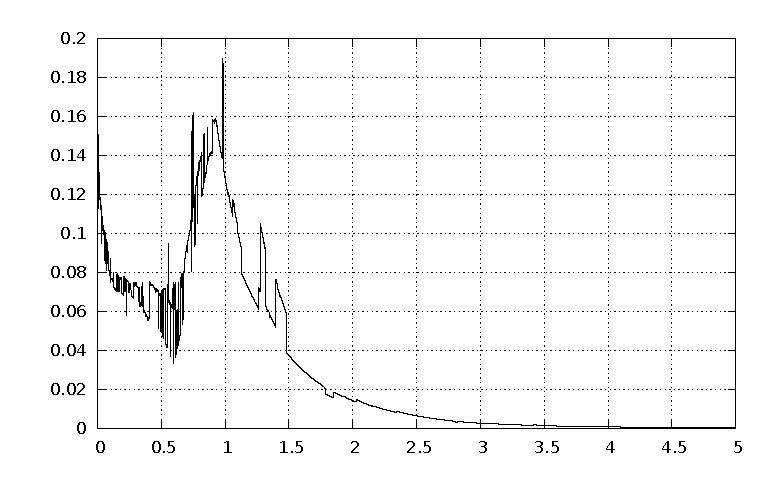
\includegraphics[width=.45\textwidth]{figures/nonuniform_bubble_velocity_remesh.ps}
  \caption{($\mu=\gamma=1$) $\|\vec U^m\|_{L^\infty(\Omega)}$ evolution of a non uniform circle formed by 64 vertices with $C_s=1$ and $C_r=3$ for the P2--P0 element, uniform mesh.}
  \label{fig:nonuniform_bubble_velocity_remesh}
\end{figure}

Instead, in Figure~\ref{fig:nonuniform_bubble_smooth} are shown some snapshots of the mesh evolution when an adaptive mesh with characteristic length $c_l=0.25$ for the boundary is used and no remeshing is performed. In Figure~\ref{fig:nonuniform_bubble_velocity_smooth} is shown the evolution of $\|\vec U^m\|_{L^\infty(\Omega)}$. Also in this case, the approximations $\Gamma^m$ converge towards an equidistributed circle, while $\vec U^m$ converges to zero.
\begin{figure}[htbp]
  \centering
  \subfloat[$t=0$]{\includegraphics[width=.45\textwidth]{figures/nonuniform_bubble_smooth_000.ps}}\\
  \subfloat[$t=0.5$]{\includegraphics[width=.45\textwidth]{figures/nonuniform_bubble_smooth_050.ps}}\quad
  \subfloat[$t=1$]{\includegraphics[width=.45\textwidth]{figures/nonuniform_bubble_smooth_100.ps}}\\
  \subfloat[$t=2.5$]{\includegraphics[width=.45\textwidth]{figures/nonuniform_bubble_smooth_250.ps}}\quad
  \subfloat[$t=5$]{\includegraphics[width=.45\textwidth]{figures/nonuniform_bubble_smooth_500.ps}}\\
  \caption{($\mu=\gamma=1$) Mesh evolution of a non uniform circle formed by 64 vertices with $C_s=1$ and no remeshing for the P2--P0 element, adaptive mesh.}
  \label{fig:nonuniform_bubble_smooth}
\end{figure}

\begin{figure}[htbp]
  \centering
  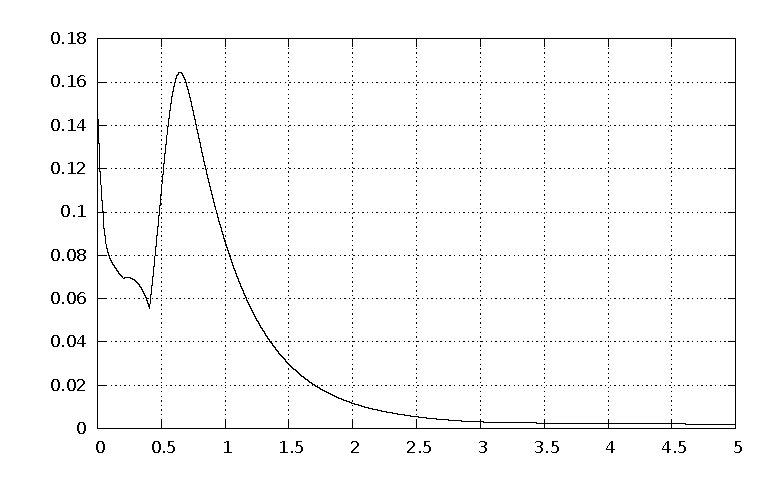
\includegraphics[width=.45\textwidth]{figures/nonuniform_bubble_velocity_smooth.ps}
  \caption{($\mu=\gamma=1$) $\|\vec U^m\|_{L^\infty(\Omega)}$ evolution of a non uniform circle formed by 64 vertices with $C_s=1$ and no remeshing for the P2--P0 element, adaptive mesh.}
  \label{fig:nonuniform_bubble_velocity_smooth}
\end{figure}

In Figure~\ref{fig:ellipse_both} is reported the pressure evolution of an ellipse, of axis 0.8 and 0.375, with initial characteristic length $c_l=0.1$, smoothing coefficient $C_s=1$ and remeshing coefficient $C_r=3$ for the P2--P0 element. We fix the usual domain $\Omega = (-1,1)^2$ and we use the parameters $\mu=1$, $\gamma=1$, $\tau=10^{-2}$ and $T=4$. The mesh is uniform and we prescribe homogeneous Dirichlet
boundary condition. Figure~\ref{fig:ellipse_both_volumes} shows the evolution of the bulk inner relative volume $\frac{\mathcal{L}^d(\Omega^h_-(t))}{\mathcal{L}^d(\Omega^h_-(0))}$ and the evolution of the interface length $\mathcal{H}^{d-1}(\Gamma^h(t))$. We point out that, since there is no exact solution to the problem, we cannot show the pressure state at $t=0$ therefore we show the pressure state at $t=10^{-5}$.
\begin{figure}[htbp]
  \centering
  \subfloat[$t=10^{-5}$]{\includegraphics[width=.45\textwidth]{figures/ellipse_both_000.ps}}\\
  \subfloat[$t=1$]{\includegraphics[width=.45\textwidth]{figures/ellipse_both_100.ps}}\quad
  \subfloat[$t=2$]{\includegraphics[width=.45\textwidth]{figures/ellipse_both_200.ps}}\\
  \subfloat[$t=3$]{\includegraphics[width=.45\textwidth]{figures/ellipse_both_300.ps}}\quad
  \subfloat[$t=4$]{\includegraphics[width=.45\textwidth]{figures/ellipse_both_400.ps}}\\
  \caption{($\mu=\gamma=1$) Pressure evolution of an ellipse with $c_l=0.1$, $C_s=1$ and $C_r=3$ for the P2--P0 element, uniform mesh.}
  \label{fig:ellipse_both}
\end{figure}

\begin{figure}[htbp]
  \centering
  \subfloat[$\frac{\mathcal{L}^d(\Omega^h_-(t))}{\mathcal{L}^d(\Omega^h_-(0))}$]{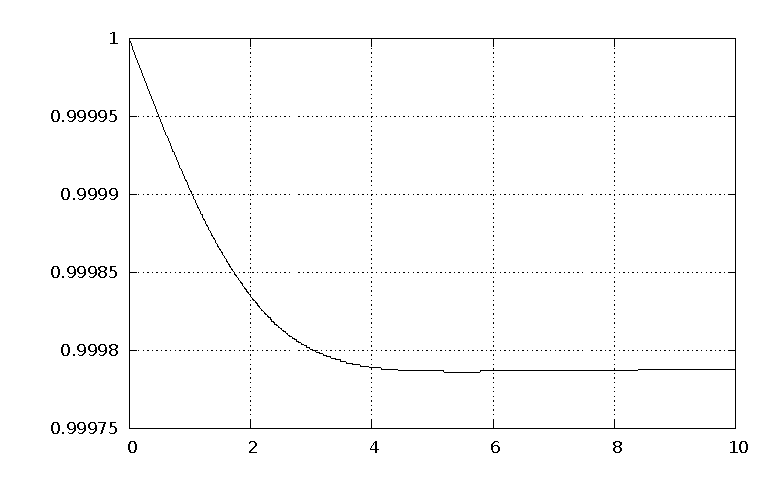
\includegraphics[width=.45\textwidth]{figures/ellipse_both_bulk_inner_volume.ps}}
  \subfloat[$\mathcal{H}^{d-1}(\Gamma^h(t))$]{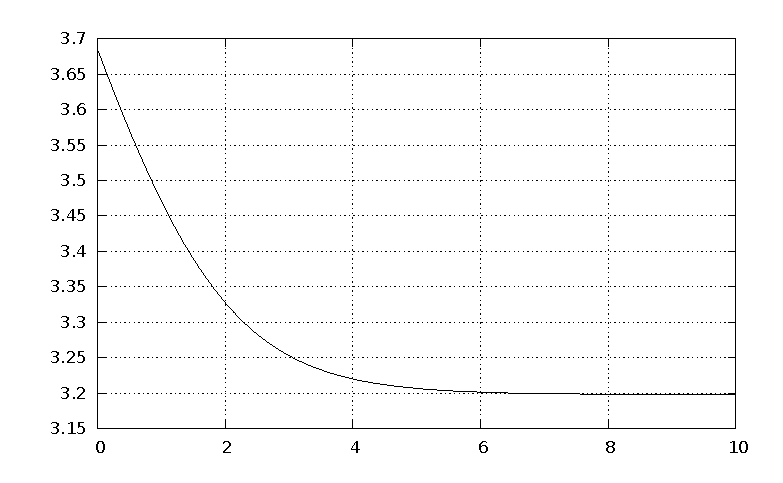
\includegraphics[width=.45\textwidth]{figures/ellipse_both_interface_length.ps}}
  \caption{($\mu=\gamma=1$) Bulk inner relative volume evolution and interface length evolution of an ellipse with $c_l=0.1$, $C_s=1$ and $C_r=3$ for the P2--P0 element, uniform mesh.}
  \label{fig:ellipse_both_volumes}
\end{figure}

Instead, in Figure~\ref{fig:ellipse_smooth} only the smoothing is used while the evolution of the bulk inner relative volume and the evolution of the interface length are shown in Figure~\ref{fig:ellipse_smooth_volumes}.
\begin{figure}[htbp]
  \centering
  \subfloat[$t=10^{-5}$]{\includegraphics[width=.45\textwidth]{figures/ellipse_smooth_000.ps}}\\
  \subfloat[$t=1$]{\includegraphics[width=.45\textwidth]{figures/ellipse_smooth_100.ps}}\quad
  \subfloat[$t=2$]{\includegraphics[width=.45\textwidth]{figures/ellipse_smooth_200.ps}}\\
  \subfloat[$t=3$]{\includegraphics[width=.45\textwidth]{figures/ellipse_smooth_300.ps}}\quad
  \subfloat[$t=4$]{\includegraphics[width=.45\textwidth]{figures/ellipse_smooth_400.ps}}\\
  \caption{($\mu=\gamma=1$) Pressure evolution of an ellipse with $c_l=0.1$, $C_s=1$ and no remeshing for the P2--P0 element, uniform mesh.}
  \label{fig:ellipse_smooth}
\end{figure}

\begin{figure}[htbp]
  \centering
  \subfloat[$\frac{\mathcal{L}^d(\Omega^h_-(t))}{\mathcal{L}^d(\Omega^h_-(0))}$]{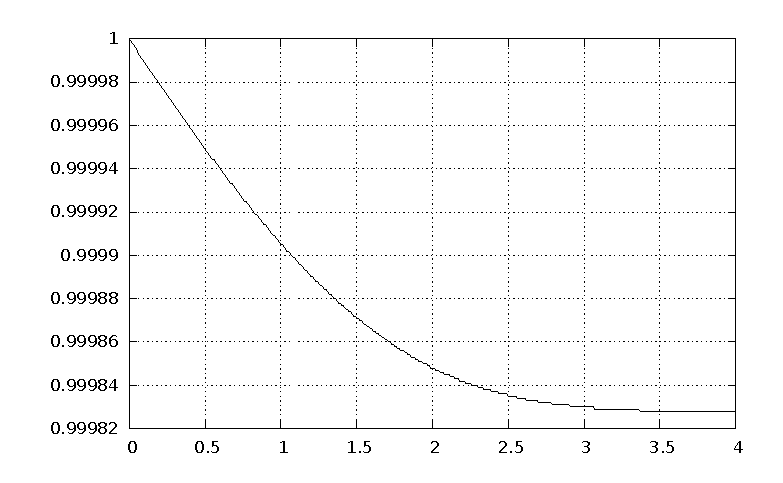
\includegraphics[width=.45\textwidth]{figures/ellipse_smooth_bulk_inner_volume.ps}}
  \subfloat[$\mathcal{H}^{d-1}(\Gamma^h(t))$]{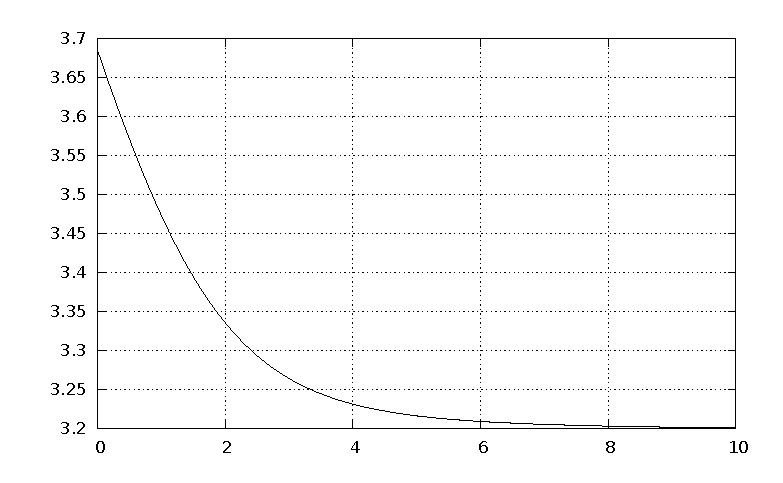
\includegraphics[width=.45\textwidth]{figures/ellipse_smooth_interface_length.ps}}
  \caption{($\mu=\gamma=1$) Bulk inner relative volume evolution and interface length evolution of an ellipse with $c_l=0.1$, $C_s=1$ and no remeshing for the P2--P0 element, uniform mesh.}
  \label{fig:ellipse_smooth_volumes}
\end{figure}

For the expanding bubble test, we fix $\Omega = (-1,1)^2 \setminus [-\frac13,\frac13]^2$ and we choose the parameters
\begin{equation*}
\alpha = 0.15 \quad\text{and}\quad \mu = \gamma = 1
\end{equation*}
for the true solution (\ref{eq:radialr2},b). In Figure~\ref{fig:expanding_bubble_uniform} is reported the pressure evolution for the expanding bubble problem with initial characteristic length $c_l=0.1$, smoothing coefficient $C_s=1$ and remeshing coefficient $C_r=3$ using an uniform mesh for the P2--P0 element.
\begin{figure}[htbp]
  \centering
  \subfloat[$t=0$]{\includegraphics[width=.45\textwidth]{figures/expanding_bubble_uniform_000.ps}}\\
  \subfloat[$t=0.25$]{\includegraphics[width=.45\textwidth]{figures/expanding_bubble_uniform_025.ps}}\quad
  \subfloat[$t=0.5$]{\includegraphics[width=.45\textwidth]{figures/expanding_bubble_uniform_050.ps}}\\
  \subfloat[$t=0.75$]{\includegraphics[width=.45\textwidth]{figures/expanding_bubble_uniform_075.ps}}\quad
  \subfloat[$t=1$]{\includegraphics[width=.45\textwidth]{figures/expanding_bubble_uniform_100.ps}}\\
  \caption{($\mu=\gamma=1,\alpha = 0.15$) Pressure evolution of the 2D expanding bubble with $c_l=0.1$, $C_s=1$ and $C_r=3$ for the P2--P0 element, uniform mesh.}
  \label{fig:expanding_bubble_uniform}
\end{figure}

In Table~\ref{tab:expandingbubble2Delements} it is reported the characteristic length $c_l$ used to create the initial mesh for the expanding bubble problem, the corresponding number of interface elements $K_\Gamma$ generated, the corresponding number of bulk elements $K_\Omega$ generated and the time step $\tau$ used. 
\begin{table*}
 \center
\begin{tabular}{llll}
\hline
$c_l$ & $K_\Gamma$ & $K_\Omega$ & $\tau$\\
\hline
0.25 & 16 & 212 & $10^{-1}$ \\
0.1 & 32 & 988 & $10^{-2}$ \\
0.05 & 64 & 3776 & $10^{-3}$ \\
\hline
\end{tabular}
\caption{Number of interface elements ($K_\Gamma$), number of bulk elements ($K_\Omega$) and time step ($\tau$) for a certain characteristic length ($c_l$) for the 2D expanding bubble problem, uniform mesh.}
\label{tab:expandingbubble2Delements}
\end{table*}

Some errors for our approximation are shown in Table~\ref{tab:expandingbubble2Dp2p0remesh} for what concern P2--P0 and in Table~\ref{tab:expandingbubble2Dp2p1p0remesh} for what concern P2--(P1+P0)  when a remeshing is performed at each time step and no smoothing is used.
\begin{table*}
 \center
\begin{tabular}{llHlHllll}
\hline
$c_l$ & $\errorXx$ & $\LerrorUu2$ & $\errorUu2$ & $\LerrorPp0$ & $\errorPp0$ & $CPU[s]$ & $K_\Omega^T$\\
\hline
0.25 & 9.59020e-03 & 5.91121e-04 & 4.09862e-03 & 1.43868e-01 & 3.72132e-01 & 36.632 & 120\\
0.1 & 1.71523e-03 & 1.07812e-04 & 8.68997e-04 & 1.84066e-02 & 4.56430e-02 & 1402.8 & 452\\
0.05 & 3.66077e-04 & 1.48787e-05 & 1.92562e-04 & 2.87838e-03 & 7.63704e-03 & 62112 & 1866\\
\hline
\end{tabular}
\caption{($\mu=\gamma=1,\alpha = 0.15$) Expanding bubble problem on $(-1,1)^2\setminus[-\frac{1}{3},\frac{1}{3}]^2$ over the time interval $[0,1]$ for the P2--P0 element, with remeshing at every time step and uniform mesh.}
\label{tab:expandingbubble2Dp2p0remesh}
\end{table*}

\ifthesis
\begin{table*}
 \center
\begin{tabular}{llHlHllll}
\hline
$c_l$ & $\errorXx$ & $\LerrorUu2$ & $\errorUu2$ & $\LerrorPp1$ & $\errorPp1$ & $CPU[s]$ & $K_\Omega^T$\\
\hline
0.25 & 6.72793e-03 & 9.18724e-03 & 2.68895e-02 & 6.57692e-01 & 1.86246e+00 & 35.519 & 120\\
0.1 & 7.86359e-03 & 4.26446e-03 & 1.53507e-02 & 4.63074e-01 & 1.83618e+00 & 1578.5 & 468\\
0.05 & 4.44456e-03 & 1.49021e-03 & 6.91841e-03 & 3.19935e-01 & 1.42542e+00 & 65958 & 1856\\
\hline
\end{tabular}
\caption{($\mu=\gamma=1,\alpha = 0.15$) Expanding bubble problem on $(-1,1)^2\setminus[-\frac{1}{3},\frac{1}{3}]^2$ over the time interval $[0,1]$ for the P2--P1 element, with remeshing at every time step and uniform mesh.}
\label{tab:expandingbubble2Dp2p1remesh}
\end{table*}
\fi

\begin{table*}
 \center
\begin{tabular}{llHlHllll}
\hline
$c_l$ & $\errorXx$ & $\LerrorUu2$ & $\errorUu2$ & $\LerrorPp{1,\rm{DG}}$ & $\errorPp{1,\rm{DG}}$ & $CPU[s]$ & $K_\Omega^T$\\
\hline
0.25 & 9.63687e-03 & 9.25039e-04 & 3.82844e-03 & 1.46701e-01 & 5.85530e-01 & 41.401 & 120\\
0.1 & 1.72931e-03 & 2.47559e-04 & 3.39462e-03 & 2.60172e-02 & 3.96317e-01 & 1578 & 452\\
0.05 & 3.66563e-04 & 2.35009e-05 & 2.72774e-04 & 3.77802e-03 & 5.76371e-02 & 75651 & 1868\\
\hline
\end{tabular}
\caption{($\mu=\gamma=1,\alpha = 0.15$) Expanding bubble problem on $(-1,1)^2\setminus[-\frac{1}{3},\frac{1}{3}]^2$ over the time interval $[0,1]$ for the P2--(P1+P0) element, with remeshing at every time step and uniform mesh.}
\label{tab:expandingbubble2Dp2p1p0remesh}
\end{table*}

Some errors for our approximation are shown in Table~\ref{tab:expandingbubble2Dp2p0smooth} for what concern P2--P0 and in Table~\ref{tab:expandingbubble2Dp2p1p0smooth} for what concern P2--(P1+P0) when a smoothing with coefficient $C_s=1$ is performed at each time step and no remeshing is used.
\begin{table*}
 \center
\begin{tabular}{llHlHlll}
\hline
$c_l$ & $\errorXx$ & $\LerrorUu2$ & $\errorUu2$ & $\LerrorPp0$ & $\errorPp0$ & $CPU[s]$\\
\hline
0.25 & 9.74956e-03 & 9.45854e-04 & 3.71046e-03 & 1.44456e-01 & 3.72132e-01 & 45.287\\
0.1 & 1.75510e-03 & 3.32420e-04 & 1.52677e-03 & 1.89573e-02 & 5.65689e-02 & 2140.7\\
0.05 & 3.86187e-04 & 8.68664e-05 & 5.33729e-04 & 4.12034e-03 & 1.73534e-02 & 125110\\
\hline
\end{tabular}
\caption{($\mu=\gamma=1,\alpha = 0.15$) Expanding bubble problem on $(-1,1)^2\setminus[-\frac{1}{3},\frac{1}{3}]^2$ over the time interval $[0,1]$ for the P2--P0 element, $C_s=1$, no remeshing and uniform mesh.}
\label{tab:expandingbubble2Dp2p0smooth}
\end{table*}

\ifthesis
\begin{table*}
 \center
\begin{tabular}{llHlHlll}
\hline
$c_l$ & $\errorXx$ & $\LerrorUu2$ & $\errorUu2$ & $\LerrorPp1$ & $\errorPp1$ & $CPU[s]$ \\
\hline
0.25 & 4.54754e-03 & 7.20725e-03 & 1.91472e-02 & 5.39278e-01 & 1.86246e+00 & 37.779\\
0.1 & 6.63921e-03 & 3.28381e-03 & 1.25620e-02 & 3.32005e-01 & 1.83618e+00 & 2145.6\\
0.05 & 3.74146e-03 & 1.23051e-03 & 6.66689e-03 & 2.15909e-01 & 1.42022e+00 & 93025\\
\hline
\end{tabular}
\caption{($\mu=\gamma=1,\alpha = 0.15$) Expanding bubble problem on $(-1,1)^2\setminus[-\frac{1}{3},\frac{1}{3}]^2$ over the time interval $[0,1]$ for the P2--P1 element, $C_s=1$, no remeshing and uniform mesh.}
\label{tab:expandingbubble2Dp2p1smooth}
\end{table*}
\fi

\begin{table*}
 \center
\begin{tabular}{llHlHlll}
\hline
$c_l$ & $\errorXx$ & $\LerrorUu2$ & $\errorUu2$ & $\LerrorPp{1,\rm{DG}}$ & $\errorPp{1,\rm{DG}}$ & $CPU[s]$\\
\hline
0.25 & 9.75830e-03 & 1.47842e-03 & 3.87930e-03 & 1.50724e-01 & 5.85530e-01 & 46.73\\
0.1 & 1.77013e-03 & 4.39215e-04 & 1.69488e-03 & 2.69416e-02 & 1.83356e-01 & 2448.5\\
0.05 & 3.78745e-04 & 1.09782e-04 & 8.91862e-04 & 7.81970e-03 & 1.10068e-01 & 108790\\
\hline
\end{tabular}
\caption{($\mu=\gamma=1,\alpha = 0.15$) Expanding bubble problem on $(-1,1)^2\setminus[-\frac{1}{3},\frac{1}{3}]^2$ over the time interval $[0,1]$ for the P2--(P1+P0) element, $C_s=1$, no remeshing and uniform mesh.}
\label{tab:expandingbubble2Dp2p1p0smooth}
\end{table*}

In order to choose the better remeshing coefficient $C_r$ several experiment were carried out. Some errors for our approximation are shown in Table~\ref{tab:expandingbubble2Dp2p0bothdiffcr} with a starting characteristic length $c_l=0.1$, using P2--P0 polynomials and smoothing coefficient $C_s=1$. The better result are obtained with $C_r=3$ because it reduces the number of remeshing compared to $C_r=2$ while keeping the same performance and error quality. For this reason we are going to use this parameter for the other simulations.
\begin{table*}
 \center
\begin{tabular}{llHlHllll}
\hline
$C_r$ & $\errorXx$ & $\LerrorUu2$ & $\errorUu2$ & $\LerrorPp0$ & $\errorPp0$ & $CPU[s]$ & $K_\Omega^T$\\
\hline
2 & 1.71500e-03 & 1.07788e-04 & 8.66903e-04 & 1.84060e-02 & 4.56430e-02 & 1494.2 & 452\\
3 & 1.72575e-03 & 1.03609e-04 & 7.19812e-04 & 1.83599e-02 & 4.56430e-02 & 1561.3 & 468\\
4 & 1.73115e-03 & 1.29324e-04 & 8.85266e-04 & 1.83974e-02 & 4.56430e-02 & 1657.7 & 504\\
5 & 1.72580e-03 & 1.03604e-04 & 7.20310e-04 & 1.83590e-02 & 4.56430e-02 & 1497.3 & 468\\
\hline
\end{tabular}
\caption{($\mu=\gamma=1,\alpha = 0.15$) Expanding bubble problem on $(-1,1)^2\setminus[-\frac{1}{3},\frac{1}{3}]^2$ over the time interval $[0,1]$ for the P2--P0 element, $C_s=1$, $c_l=0.1$ and uniform mesh.}
\label{tab:expandingbubble2Dp2p0bothdiffcr}
\end{table*}

Some errors for our approximation are shown in Table~\ref{tab:expandingbubble2Dp2p0all} for what concern P2--P0 and in Table~\ref{tab:expandingbubble2Dp2p1p0all} for what concern P2--(P1+P0) whit remeshing coefficient $C_r=3$ and with smoothing coefficient $C_s=1$.
\begin{table*}
 \center
\begin{tabular}{llHlHllll}
\hline
$c_l$ & $\errorXx$ & $\LerrorUu2$ & $\errorUu2$ & $\LerrorPp0$ & $\errorPp0$ & $CPU[s]$ & $K_\Omega^T$\\
\hline
0.25 & 9.54922e-03 & 8.91817e-04 & 3.28947e-03 & 1.45205e-01 & 3.72132e-01 & 44.892 & 184\\
0.1 & 1.72575e-03 & 1.03609e-04 & 7.19812e-04 & 1.83599e-02 & 4.56430e-02 & 1561.3 & 468\\
0.05 & 3.66047e-04 & 1.50674e-05 & 1.74840e-04 & 2.88134e-03 & 7.63707e-03 & 63215 & 1864\\
\hline
\end{tabular}
\caption{($\mu=\gamma=1,\alpha = 0.15$) Expanding bubble problem on $(-1,1)^2\setminus[-\frac{1}{3},\frac{1}{3}]^2$ over the time interval $[0,1]$ for the P2--P0 element, $C_s=1$, $C_r=3$ and uniform mesh.}
\label{tab:expandingbubble2Dp2p0all}
\end{table*}

\ifthesis
\begin{table*}
 \center
\begin{tabular}{llHlHllll}
\hline
$c_l$ & $\errorXx$ & $\LerrorUu2$ & $\errorUu2$ & $\LerrorPp1$ & $\errorPp1$ & $CPU[s]$ & $K_\Omega^T$\\
\hline
0.25 & 6.69114e-03 & 9.11156e-03 & 2.72737e-02 & 6.48539e-01 & 1.86246e+00 & 35.888 & 164\\
0.1 & 7.47170e-03 & 3.94367e-03 & 1.51501e-02 & 4.24146e-01 & 1.83618e+00 & 1718.3 & 468\\
0.05 & 4.38718e-03 & 1.46440e-03 & 7.06896e-03 & 3.10958e-01 & 1.42542e+00 & 60968 & 1864\\
\hline
\end{tabular}
\caption{($\mu=\gamma=1,\alpha = 0.15$) Expanding bubble problem on $(-1,1)^2\setminus[-\frac{1}{3},\frac{1}{3}]^2$ over the time interval $[0,1]$ for the P2--P1 element, $C_s=1$, $C_r=3$ and uniform mesh.}
\label{tab:expandingbubble2Dp2p1all}
\end{table*}
\fi

\begin{table*}
 \center
\begin{tabular}{llHlHllll}
\hline
$c_l$ & $\errorXx$ & $\LerrorUu2$ & $\errorUu2$ & $\LerrorPp{1,\rm{DG}}$ & $\errorPp{1,\rm{DG}}$ & $CPU[s]$ & $K_\Omega^T$\\
\hline
0.25 & 9.67194e-03 & 9.20512e-04 & 3.73007e-03 & 1.46187e-01 & 5.85530e-01 & 46.025 & 184\\
0.1 & 1.73742e-03 & 2.23657e-04 & 2.82615e-03 & 2.51153e-02 & 4.02237e-01 & 1794.2 & 468\\
0.05 & 3.66901e-04 & 2.35815e-05 & 2.15554e-04 & 3.76150e-03 & 5.82683e-02 & 71301 & 1864\\
\hline
\end{tabular}
\caption{($\mu=\gamma=1,\alpha = 0.15$) Expanding bubble problem on $(-1,1)^2\setminus[-\frac{1}{3},\frac{1}{3}]^2$ over the time interval $[0,1]$ for the P2--(P1+P0) element, $C_s=1$, $C_r=3$ and uniform mesh.}
\label{tab:expandingbubble2Dp2p1p0all}
\end{table*}

In all the previous simulations, the meshes used were uniform therefore the characteristic length was equal for all the nodes. Moreover they were kept uniform also after the remeshing. Obviously, with this approach, it is very expensive to have a large number of interface elements since it leads to a drastic increase of bulk elements. In the following simulations, instead, we use adaptive meshes which are fine close to the interface and coarse far from the interface. In Figure~\ref{fig:expanding_bubble_adaptive} is reported the pressure evolution for the expanding bubble problem with an adaptive mesh which has characteristic interface length $c_{l,\Gamma}=0.05$ for the P2--P0 element. This time no smoothing is performed since we need to remesh at each time step.
\begin{figure}[htbp]
  \centering
  \subfloat[$t=0$]{\includegraphics[width=.45\textwidth]{figures/expanding_bubble_adaptive_000.ps}}\\
  \subfloat[$t=0.25$]{\includegraphics[width=.45\textwidth]{figures/expanding_bubble_adaptive_025.ps}}\quad
  \subfloat[$t=0.5$]{\includegraphics[width=.45\textwidth]{figures/expanding_bubble_adaptive_050.ps}}\\
  \subfloat[$t=0.75$]{\includegraphics[width=.45\textwidth]{figures/expanding_bubble_adaptive_075.ps}}\quad
  \subfloat[$t=1$]{\includegraphics[width=.45\textwidth]{figures/expanding_bubble_adaptive_100.ps}}\\
  \caption{($\mu=\gamma=1,\alpha = 0.15$) Pressure evolution of the 2D expanding bubble with $c_l=0.1$, with remeshing at every time step for the P2--P0 element, adaptive mesh.}
  \label{fig:expanding_bubble_adaptive}
\end{figure}

The characteristic length of the bulk elements, $c_{l,\Omega}(\vec{x})$, is computed as
\begin{equation}\label{eq:adaptive_criteria}
 c_{l,\Omega}(\vec{x})=\min\big\{8c_{l,\Gamma},\textrm{dist}(\vec{x},\Gamma)\big\}
\end{equation}
where $\vec{x}\in\partial\Omega$ is a mesh node. See Table~\ref{tab:expandingbubble2Delements_adaptive} for the resulting number of elements. 
\begin{table*}
 \center
\begin{tabular}{llll}
\hline
$c_{l,\Gamma}$ & $K_\Gamma$ & $K_\Omega$ & $\tau$ \\
\hline
0.05 & 64 & 1020 & $1.6\cdot10^{-2}$ \\
0.025 & 128 & 2506 & $4\cdot10^{-3}$\\
0.0123 & 256 & 7460 & $10^{-3}$\\
\hline
\end{tabular}
\caption{Number of interface elements ($K_\Gamma$), number of bulk elements ($K_\Omega$) and time step ($\tau$) for a certain characteristic length ($c_l$) for the 2D expanding bubble problem, adaptive mesh.}
\label{tab:expandingbubble2Delements_adaptive}
\end{table*}

Some errors for our approximation are shown in Table~\ref{tab:expandingbubble2Dp2p0adaptive} for what concern P2--P0 and in Table~\ref{tab:expandingbubble2Dp2p1p0adaptive} for what concern P2--(P1+P0).
\begin{table*}
 \center
\begin{tabular}{llHlHllll}
\hline
$c_l$ & $\errorXx$ & $\LerrorUu2$ & $\errorUu2$ & $\LerrorPp0$ & $\errorPp0$ & $CPU[s]$ & $K_\Omega^T$\\
\hline
0.05 & 1.00492e-03 & 3.65898e-04 & 1.84254e-03 & 2.17526e-02 & 4.75296e-02 & 537.01 & 564\\
0.25 & 2.65031e-04 & 2.81870e-04 & 2.60458e-03 & 8.19573e-03 & 5.09886e-02 & 8686.3 & 1232\\
0.0123 & 6.15383e-05 & 6.98648e-05 & 6.90439e-04 & 2.38225e-03 & 1.50292e-02 & 119900 & 3860\\
\hline
\end{tabular}
\caption{($\mu=\gamma=1,\alpha = 0.15$) Expanding bubble problem on $(-1,1)^2\setminus[-\frac{1}{3},\frac{1}{3}]^2$ over the time interval $[0,1]$ for the P2--P0 element, with remeshing at every time step and adaptive mesh.}
\label{tab:expandingbubble2Dp2p0adaptive}
\end{table*}

\ifthesis
\begin{table*}
 \center
\begin{tabular}{llHlHllll}
\hline
$c_l$ & $\errorXx$ & $\LerrorUu2$ & $\errorUu2$ & $\LerrorPp1$ & $\errorPp1$ & $CPU[s]$ & $K_\Omega^T$\\
\hline
0.05 & 5.83738e-03 & 2.53548e-03 & 1.02947e-02 & 4.02004e-01 & 1.55842e+00 & 539.24 & 546\\
0.025 & 2.96051e-03 & 9.44063e-04 & 5.17811e-03 & 2.54813e-01 & 1.46784e+00 & 8499.5 & 1212\\
0.0123 & 1.44126e-03 & 2.99560e-04 & 2.32296e-03 & 1.70133e-01 & 1.48891e+00 & 114050 & 3856\\
\hline
\end{tabular}
\caption{($\mu=\gamma=1,\alpha = 0.15$) Expanding bubble problem on $(-1,1)^2\setminus[-\frac{1}{3},\frac{1}{3}]^2$ over the time interval $[0,1]$ for the P2--P1 element, with remeshing at every time step and adaptive mesh.}
\label{tab:expandingbubble2Dp2p1adaptive}
\end{table*}
\fi

\begin{table*}
 \center
\begin{tabular}{llHlHllll}
\hline
$c_l$ & $\errorXx$ & $\LerrorUu2$ & $\errorUu2$ & $\LerrorPp{1,\rm{DG}}$ & $\errorPp{1,\rm{DG}}$ & $CPU[s]$ & $K_\Omega^T$\\
\hline
0.05 & 1.07834e-03 & 6.59317e-04 & 3.26722e-03 & 3.20463e-02 & 3.07658e-01 & 631.62 & 564\\
0.025 & 3.18849e-04 & 5.16850e-04 & 3.13403e-03 & 2.21693e-02 & 3.07668e-01 & 10836 & 1236\\
0.0123 & 7.67770e-05 & 1.56422e-04 & 1.63225e-03 & 1.05762e-02 & 1.61938e-01 & 133400 & 3866\\
\hline
\end{tabular}
\caption{($\mu=\gamma=1,\alpha = 0.15$) Expanding bubble problem on $(-1,1)^2\setminus[-\frac{1}{3},\frac{1}{3}]^2$ over the time interval $[0,1]$ for the P2--(P1+P0) element, with remeshing at every time step and adaptive mesh.}
\label{tab:expandingbubble2Dp2p1p0adaptive}
\end{table*}

Finally, we report a shear flow in the domain $\Omega=(-1,1)^2$, with a circle of radius $r=0.5$ as initial interface. We prescribe the inhomogeneous Dirichlet boundary condition
\begin{equation*}
\vec g(\vec z)=(z_2,0)^T\quad \mbox{on }\partial\Omega\,,
\end{equation*}
and we use the parameters $\mu=1$, $\gamma=3$, $\tau=10^{-2}$ and $T=5$. In Figure~\ref{fig:shear_2d} is reported the pressure evolution using a characteristic length $c_l=0.05$ and an uniform mesh, smoothing coefficient $C_s=1$ and remeshing coefficient $C_r=3$ for the P2--P0 element. In Figure~\ref{fig:shear_2d_velocity} is shown the velocity vector field evolution while the bulk inner relative volume evolution $\frac{\mathcal{L}^d(\Omega^h_-(t))}{\mathcal{L}^d(\Omega^h_-(0))}$ is reported in Figure~\ref{fig:shear_2d_bulk_inner_volume}.
\begin{figure}[htbp]
  \centering
  \subfloat[$t=0.5$]{\includegraphics[width=.45\textwidth]{figures/2d_shear_050.ps}}\quad
  \subfloat[$t=1$]{\includegraphics[width=.45\textwidth]{figures/2d_shear_100.ps}}\\
  \subfloat[$t=2.5$]{\includegraphics[width=.45\textwidth]{figures/2d_shear_250.ps}}\quad
  \subfloat[$t=5$]{\includegraphics[width=.45\textwidth]{figures/2d_shear_500.ps}}\\
  \caption{($\mu=1,\gamma=3$) Pressure evolution of the 2D shear flow with $c_l=0.05$, $C_s=1$ and $C_r=3$ for the P2--P0 element, uniform mesh.}
  \label{fig:shear_2d}
\end{figure}

\begin{figure}[htbp]
  \centering
  \subfloat[$t=0.5$]{\includegraphics[width=.45\textwidth]{figures/2d_shear_velocity_050.ps}}\quad
  \subfloat[$t=1$]{\includegraphics[width=.45\textwidth]{figures/2d_shear_velocity_100.ps}}\\
  \subfloat[$t=2.5$]{\includegraphics[width=.45\textwidth]{figures/2d_shear_velocity_250.ps}}\quad
  \subfloat[$t=5$]{\includegraphics[width=.45\textwidth]{figures/2d_shear_velocity_500.ps}}\\
  \caption{($\mu=1,\gamma=3$) Velocity vector field of the 2D shear flow with $c_l=0.05$, $C_s=1$ and $C_r=3$ for the P2--P0 element, uniform mesh.}
  \label{fig:shear_2d_velocity}
\end{figure}

\begin{figure}[htbp]
  \centering
  \includegraphics[width=.45\textwidth]{figures/2d_shear_bulk_inner_volume.ps}
  \caption{($\mu=\gamma=1$) Bulk inner relative volume evolution of the 2D shear flow with $c_l=0.05$, $C_s=1$ and $C_r=3$ for the P2--P0 element, uniform mesh.}
  \label{fig:shear_2d_bulk_inner_volume}
\end{figure}

Instead, in Figure~\ref{fig:shear_2d_smooth} the remeshing coefficient is $C_r=0$ so only the smoothing is used. The bulk inner relative volume evolution is reported in Figure~\ref{fig:shear_2d_smooth_bulk_inner_volume}.
\begin{figure}[htbp]
  \centering
  \subfloat[$t=0.5$]{\includegraphics[width=.45\textwidth]{figures/2d_shear_smooth_050.ps}}\quad
  \subfloat[$t=1$]{\includegraphics[width=.45\textwidth]{figures/2d_shear_smooth_100.ps}}\\
  \subfloat[$t=2.5$]{\includegraphics[width=.45\textwidth]{figures/2d_shear_smooth_250.ps}}\quad
  \subfloat[$t=5$]{\includegraphics[width=.45\textwidth]{figures/2d_shear_smooth_500.ps}}\\
  \caption{($\mu=1,\gamma=3$) Pressure evolution of the 2D shear flow with $c_l=0.05$, $C_s=1$ and no remeshing for the P2--P0 element, uniform mesh.}
  \label{fig:shear_2d_smooth}
\end{figure}

\begin{figure}[htbp]
  \centering
  \includegraphics[width=.45\textwidth]{figures/2d_shear_smooth_bulk_inner_volume.ps}
  \caption{($\mu=\gamma=1$) Bulk inner relative volume evolution of the 2D shear flow with $c_l=0.05$, $C_s=1$ and no remeshing for the P2--P0 element, uniform mesh.}
  \label{fig:shear_2d_smooth_bulk_inner_volume}
\end{figure}

\subsection{Numerical results in 3d} \label{subsec:numerical_results_3d}
\setcounter{equation} 0

For the stationary bubble test we use the domain $\Omega = (-1,1)^3$ and we choose, for the true solution (\ref{eq:radialr},b), the parameters
\begin{equation*}
\mu = \gamma = 1\,. 
\end{equation*}
Therefore, the true solution reduces to $r(t) = \frac{1}{2}$, $\vec u(\cdot, t) = \vec 0$ and $p(t) = 4\,\charfcn{\Omega_-(0)} - \frac{\pi}{12}$ for all $t\geq0$.

In Table~\ref{tab:bubble3Delements} it is reported the characteristic length $c_l$, which prescribes the desired size of the elements, used to create the mesh for the stationary bubble problem, the corresponding number of interface elements $K_\Gamma$ generated, the corresponding number of bulk elements $K_\Omega$ generated and the time step $\tau$ used. The interface mesh is obtained applying a surface diffusion to a sphere until the surface is stationary which means until the displacement is 0 up to machine accuracy for all the nodes. The bulk mesh is uniform.
\begin{table*}
 \center
\begin{tabular}{llll}
\hline
$c_l$ & $K_\Gamma$ & $K_\Omega$ & $\tau$ \\
\hline
0.5 & 32 & 408 & $10^{-2}$ \\
0.25 & 220 & 3590 & $10^{-2}$\\
0.125 & 596 & 20473 & $10^{-2}$\\
\hline
\end{tabular}
\caption{Number of interface elements ($K_\Gamma$), number of bulk elements ($K_\Omega$) and time step ($\tau$) for a certain characteristic length ($c_l$) for the 3D stationary bubble problem, stationary uniform mesh.}
\label{tab:bubble3Delements}
\end{table*}

Since the solution is stationary, neither smoothing nor remeshing is performed. 

Some errors for our numerical scheme can be seen in Table~\ref{tab:bubble3Dp2p0} for the P2--P0 element and in Table~\ref{tab:bubble3Dp2p1p0} for the P2--(P1+P0). 
\begin{table*}
 \center
\begin{tabular}{llHlHlll}
\hline
$c_l$ & $\errorXx$ & $\LerrorUu2$ & $\errorUu2$ & $\LerrorPp0$ & $\errorPp0$ & $CPU[s]$ \\
\hline
0.5 & 2.97986e-02 & 0 & 0 & 4.68089e-01 & 7.43095e-01 & 376.87\\
0.25 & 5.80971e-03 & 0 & 0 & 7.80486e-02 & 1.06521e-01 & 7173.9\\
0.125 & 2.42857e-03 & 0 & 0 & 2.86154e-02 & 3.83704e-02 & 84878 \\
\hline
\end{tabular}
\caption{($\mu=\gamma=1$) Stationary bubble problem on $(-1,1)^3$ over the time interval $[0,1]$ for the P2--P0 element, stationary uniform mesh.}
\label{tab:bubble3Dp2p0}
\end{table*}

\ifthesis
\begin{table*}
 \center
\begin{tabular}{llHlHlll}
\hline
$c_l$ & $\errorXx$ & $\LerrorUu2$ & $\errorUu2$ & $\LerrorPp1$ & $\errorPp1$ & $CPU[s]$ \\
\hline
0.5 & 1.34231e-01 & 5.95039e-02 & 1.04966e-01 & 3.54657e+00 & 8.81248e+00 & 358.11\\
0.25 & 7.60042e-02 & 3.14735e-02 & 7.26802e-02 & 1.94421e+00 & 3.75606e+00 & 2762.3\\
0.125 & 4.03084e-02 & 1.34315e-02 & 4.30264e-02 & 1.38833e+00 & 3.73339e+00 & 33051\\
\hline
\end{tabular}
\caption{($\mu=\gamma=1$) Stationary bubble problem on $(-1,1)^3$ over the time interval $[0,1]$ for the P2--P1 element, stationary uniform mesh.}
\label{tab:bubble3Dp2p1}
\end{table*}
\fi

\begin{table*}
 \center
\begin{tabular}{llHlHlll}
\hline
$c_l$ & $\errorXx$ & $\LerrorUu2$ & $\errorUu2$ & $\LerrorPp{1,\rm{DG}}$ & $\errorPp{1,\rm{DG}}$ & $CPU[s]$ \\
\hline
0.5 & 2.97986e-02 & 0 & 0 & 4.72706e-01 & 7.44770e-01 & 373.13\\
0.25 & 5.80971e-03 & 0 & 0 & 8.28392e-02 & 2.91977e-01 & 7179.5\\
0.125 & 2.42857e-03 & 0 & 0 & 3.23297e-02 & 3.10695e-01 & 124800\\
\hline
\end{tabular}
\caption{($\mu=\gamma=1$) Stationary bubble problem on $(-1,1)^3$ over the time interval $[0,1]$ for the P2--(P1+P0) element, stationary uniform mesh.}
\label{tab:bubble3Dp2p1p0}
\end{table*}

We see that the radius error in Table~\ref{tab:bubble3Dp2p0} is terrible compared to the analogous test in 2D. The reason is that in 2D the initial discrete interface is equidistributed and its radius is exactly 0.5 while in 3D the mesh is equidistributed but the initial radius has already an error. This error is exactly the one seen in the table since the displacement is always 0 up to machine accuracy. 

Finally, we report a shear flow in the domain $\Omega=(-1,1)^3$, with a sphere of radius $r=0.5$ as initial interface. The initial interface mesh is a non-stationary sphere while the bulk mesh is uniform. We prescribe the inhomogeneous Dirichlet boundary condition
\begin{equation*}
\vec g(\vec z)=(z_3,0,0)^T\quad \mbox{on }\partial\Omega\,,
\end{equation*}
and we use the parameters $\mu=1$, $\gamma=3$, $\tau=10^{-2}$ and $T=5$. In Figure~\ref{fig:shear_3d} is reported the interface evolution of the sphere with initial characteristic length $c_l=0.125$, smoothing coefficient $C_s=1$ and remeshing coefficient $C_r=3$ for the P2--P0 element. The characteristic length for the boundary is fixed and not uniform like in the 2D case. In Figure~\ref{fig:shear_3d_velocity} is shown the velocity vector field evolution in the plane normal to $(0,1,0)$ and passing through the origin while the bulk inner relative volume evolution $\frac{\mathcal{L}^d(\Omega^h_-(t))}{\mathcal{L}^d(\Omega^h_-(0))}$ is reported in Figure~\ref{fig:shear_3d_bulk_inner_volume}.
\begin{figure}[htbp]
  \centering
  \subfloat[$t=0$]{\includegraphics[width=.45\textwidth]{figures/3d_shear_000.ps}}\\
  \subfloat[$t=0.5$]{\includegraphics[width=.45\textwidth]{figures/3d_shear_050.ps}}\quad
  \subfloat[$t=1$]{\includegraphics[width=.45\textwidth]{figures/3d_shear_100.ps}}\\
  \subfloat[$t=2.5$]{\includegraphics[width=.45\textwidth]{figures/3d_shear_250.ps}}\quad
  \subfloat[$t=5$]{\includegraphics[width=.45\textwidth]{figures/3d_shear_500.ps}}\\
  \caption{($\mu=1,\gamma=3$) Interface evolution of the 3D shear flow with $c_l=0.125$, $C_s=1$ and $C_r=3$ for the P2--P0 element, uniform mesh.}
  \label{fig:shear_3d}
\end{figure}

\begin{figure}[htbp]
  \centering
  \subfloat[$t=0.5$]{\includegraphics[width=.45\textwidth]{figures/3d_shear_velocity_050.ps}}\quad
  \subfloat[$t=1$]{\includegraphics[width=.45\textwidth]{figures/3d_shear_velocity_100.ps}}\\
  \subfloat[$t=2.5$]{\includegraphics[width=.45\textwidth]{figures/3d_shear_velocity_250.ps}}\quad
  \subfloat[$t=5$]{\includegraphics[width=.45\textwidth]{figures/3d_shear_velocity_500.ps}}\\
  \caption{($\mu=1,\gamma=3$) Velocity vector field in the plane normal to $(0,1,0)$ and passing through the origin of the 3D shear flow with $c_l=0.125$, $C_s=1$ and $C_r=3$ for the P2--P0 element, uniform mesh.}
  \label{fig:shear_3d_velocity}
\end{figure}

\begin{figure}[htbp]
  \centering
  \includegraphics[width=.45\textwidth]{figures/3d_shear_bulk_inner_volume.ps}
  \caption{($\mu=\gamma=1$) Bulk inner relative volume evolution of the 3D shear flow with $c_l=0.125$, $C_s=1$ and $C_r=3$ for the P2--P0 element, uniform mesh.}
  \label{fig:shear_3d_bulk_inner_volume}
\end{figure}

\section{Conclusion}\label{sec:conclusion}
\textcolor{magenta}{TODO : add comparison reults unfitted scheme scheme stokes paper}

The P2--P0 element has the same accuracy of the P2--(P1+P0) element but it is simpler to implement, always satisfies the LBB condition and the resulting linear system is smaller therefore it is the best choice.

The adaptive mesh works very well for the stationary bubble problem. Indeed, with a fraction of bulk elements, it reaches the same accuracy of the uniform mesh. Unfortunately this is not the case for the expanding bubble problem. For this problem, the uniform mesh is much faster and requires less bulk elements compared to the adaptive mesh therefore.\footnote{But they have different $\tau$!}

In the 2D expanding bubble problem, We can observe that the simulations which use only the smoothing have bigger errors and take more time therefore it is not feasible to use only the smoothing process. On the other side both only remeshing and smoothing/remeshing combined achieve almost the same quality and performance. It is important to notice that the performance are almost the same for sequential code (our case) but in parallel computation the remeshing is the real bottleneck therefore it is way better to use the combined smoothing/remeshing approach.

Both element capture perfectly the jump in the pressure.
\newpage
\bibliographystyle{siam} 
\bibliography{../bib/robert_refs,../bib/marco_refs}
\end{document}